\documentclass[%
reprint,
 prd,
superscriptaddress,
nofootinbib,
aps,
dvipsnames
]{revtex4-2}
\usepackage[utf8]{inputenc}

\usepackage{amsmath, amsthm, amsfonts,  amssymb, latexsym}
\usepackage{graphicx}
\usepackage{dcolumn}
\usepackage{bm}
\usepackage{hyperref}
\usepackage[mathlines]{lineno}
\usepackage{orcidlink}
%\usepackage[normalem]{ulem}
\usepackage{breakurl}
% PZ: some DOIs in MyReferences.bib contain underscores, which
% apsrev typesets in text mode and which abort the build.
\usepackage{underscore}


%Only for editing: COMMENT {ULEM} AFTER EDITS
\usepackage[normalem]{ulem}
\usepackage{xcolor}
\newcommand{\PZ}[1]{\textcolor{red}{\textsf{[PZ: #1]}}}
\newcommand{\srg}[1]{\textcolor{Green}{[(Stephen) #1]}}
\newcommand{\edit}[1]{\textcolor{Orange}{#1}}
\newcommand{\CI}[1]{\textcolor{purple}{\textsf{ #1}}}
\newcommand{\SH}[1]{\textcolor{purple}{\textsf{[Change: #1]}}}

%%%%%%% Useful Packages
\usepackage{enumerate}
\usepackage{mathrsfs}
\usepackage{graphicx}

\usepackage{subcaption}
\usepackage{xfrac}
\usepackage{lmodern}
\usepackage{multirow}

\usepackage{tikz}
\usetikzlibrary{angles,
                quotes}

%%%%%%% Shortcuts
\newcommand{\bphi}{\bar \phi}
\newcommand{\bx}{\bar x}
\newcommand{\bt}{\bar t}
\newcommand{\ri}{\mathrm{in}}
\newcommand{\ru}{\mathrm{up}}
\newcommand{\vol}{\mathrm{vol}}
\newcommand{\ud}{\mathrm{d}}
\newcommand{\Lie}{{\mathcal L}}
\DeclareMathOperator*{\SumInt}{%
	\mathchoice%
	{\ooalign{$\displaystyle\sum$\cr\hidewidth$\displaystyle\int$\hidewidth\cr}}
	{\ooalign{\raisebox{.14\height}{\scalebox{.7}{$\textstyle\sum$}}\cr\hidewidth$\textstyle\int$\hidewidth\cr}}
	{\ooalign{\raisebox{.2\height}{\scalebox{.6}{$\scriptstyle\sum$}}\cr$\scriptstyle\int$\cr}}
	{\ooalign{\raisebox{.2\height}{\scalebox{.6}{$\scriptstyle\sum$}}\cr$\scriptstyle\int$\cr}}
}

% mode indices
\newcommand{\emm}{m}
\newcommand{\ess}{s}
\def\wlm{\ell \emm \omega}

%Theorems
\newtheorem{proposition}{Proposition}[section]
\newtheorem{theorem}[proposition]{Theorem}
\newtheorem{lemma}[proposition]{Lemma}
\newtheorem{conjecture}[proposition]{Conjecture}
\newtheorem{corollary}[proposition]{Corollary}
\newtheorem{definition}[proposition]{Definition}
\newtheorem{example}[proposition]{Example}
\newtheorem{remark}[proposition]{Remark}

% double angle brackets
\newcommand{\llangle}{\langle\langle}
\newcommand{\rrangle}{\rangle\rangle}

% Held scalars
%
\renewcommand{\H}[1]{{#1}^{\circ}}
\newcommand{\Held}[1]{{#1}^{\circ}}
\def\tah{{\tau}^\circ}
\def\tabh{{\bar\tau}^\circ}
\def\tauH{\tau^{\circ}}
\def\taubH{\bar{\tau}^{\circ}}
\def\Psih{ {\Psi}^\circ}
\def\Psibh{ {\bar{\Psi}}^\circ}
\def\PsiH{\Psi^{\circ}}
\def\PsibH{\bar\Psi^{\circ}}
\def\rhoph{{\rho}^{\prime \circ} }
\def\rhopH{\rho^{\prime \circ}}
\def\rhopbh{{\bar\rho}^{\prime \circ} }
\def\tauHsq{\tau^{\circ}{}^{2}}
\def\Oh{{\Omega}^\circ}

% Nicer looking GHP Ops FROM GHZ PAPER
\font\ec=ecrm0800 at 12pt
\def\thpH{\tilde{\th}'}
\def\edthH{\tilde\edth}
\def\edthpH{\tilde\edth'}
\def\th{\hbox{\ec\char'336}}
\def\edth{\hbox{\ec\char'360}}
\def\thp{\hbox{\ec\char'336}'}
\def\edthp{\hbox{\ec\char'360}'}
\def\Dbar{\tilde \edth} % Held edth
\def\Nbar{\tilde \th'}
\def\Edth{\hat{\edth}} % raising operator
\def\EdthBar{\bar{\Edth}} % lowering operator on sYlm

% Calligraphic letters
\renewcommand{\S}{{\mathcal S}}
\newcommand{\E}{{\mathcal E}}
\newcommand{\T}{{\mathcal T}}
\renewcommand{\L}{{\mathcal L}}
\renewcommand{\O}{{\mathcal O}}
\renewcommand{\P}{{\mathcal P}}
\newcommand{\A}{{\mathcal A}}

\newcommand{\sM}{{\mathscr M}}
\newcommand{\sS}{{\mathscr S}}
\newcommand{\sI}{{\mathscr I}}
\newcommand{\sH}{{\mathscr H}}
\newcommand{\sP}{{\mathscr P}}
\newcommand{\sL}{{\mathscr L}}
\newcommand{\sV}{{\mathscr V}}
\newcommand{\sW}{{\mathscr W}}
\newcommand{\sY}{{\mathscr Y}}
\newcommand{\sE}{{\mathscr E}}
\newcommand{\sX}{{\mathscr X}}
\newcommand{\sU}{{\mathscr U}}




% Group/algebra characters
\def\SLg{\ensuremath{\mathrm{SL}_2(\mathbb R)}}
\def\Ug{\ensuremath{\mathrm{U(1)}}}
\def\sla{\ensuremath{\mathfrak{sl}_2(\mathbb R)}}
\def\ua{\ensuremath{\mathfrak{sl}_2(\mathbb R)}}



%%%%%%% GHP Related
\def\F{\ensuremath{F}} % generic GHP scalar
%\DeclareMathOperator{\thorn}{\text{\th}}
\let\edth\relax
%\DeclareMathOperator{\eth}{\text{\dh}}

\font\ec=ecrm0800 at 12pt
\def\th{\hbox{\ec\char'336}}
\def\edth{\hbox{\ec\char'360}}
\def\thp{\hbox{\ec\char'336}'}
\def\edthp{\hbox{\ec\char'360}'}
\def\Dbar{\tilde \edth}
\def\Nbar{\tilde \th'}
\def\mb{\bar m}

\newcommand{\GHPLie}{\text{\L}}
\newcommand{\lie}[1]{\mathcal{L}_#1}
\newcommand{\covlie}[1]{\L{}_#1}

\def\pheq{\phantom{=}}

\DeclareMathOperator{\thorn}{\text{\rm \th}}
\let\eth\relax
\DeclareMathOperator{\eth}{\text{\rm \dh}}

\def\GHPwt{\ensuremath{\circeq}}
\newcommand{\GHPw}[2]{\left\{ #1, #2 \right\}}

% Modes
\def\Sh{\ensuremath{{}_s S_{\ell m \omega}}}
\def\Rh{\ensuremath{ {}_s R_{\ell m \omega }}}
\newcommand{\Rq}[1]{\ensuremath{ {}_s R_{\ell m #1 }}}
\def\Eh{\ensuremath{ {}_s  \mathscr{L}_{\ell m \omega}}}
\def\Kh{\ensuremath{ {}_s  K_{\ell m \omega}}}
\def\Ih{\ensuremath{ {}_s I_{\ell m \omega}}}
\def\In{\ensuremath{ {}_s I_{\ell m n}}}
\def\Ihz{\ensuremath{ {}_s I_{\ell m}}}

\def\U{\ensuremath{\Upsilon}}
\def\Us{\ensuremath{\Upsilon_{s}}}
\def\tUs{\ensuremath{\hat \Upsilon_{s}}}
\def\tUslm{\ensuremath{{}_s \hat \Upsilon_{\ell m}}}

% Standard operators
\renewcommand{\Re}{\operatorname{Re}}
\renewcommand{\Im}{\operatorname{Im}}

% Differential operators
\def\pd{\partial}          % PZ: used by the Teukolsky equations in Sec. V D
\def\half{\tfrac{1}{2}}    % PZ: likewise
\newcommand{\dd}{{\rm d}}
\newcommand{\cX}{\mathcal X}

\def\no{\nonumber \\}
\def\non{\nonumber \\}   % PZ: used in App. \ref{app:Lie}; was undefined

% =====================================================================
%  NEW MACROS ADDED FOR THIS DRAFT
% =====================================================================
% angular eigenvalue combinations
\def\l{\ensuremath{\ell}}                          % PZ: \l was undefined (LaTeX's Polish l)
\newcommand{\Bco}[1]{{}_{#1}B_{\ell}}                 % Schwarzschild  {}_sB_l
\newcommand{\BcoK}[3]{{}_{#1}B_{#2}(#3)}            % Kerr  {}_sB_{lm}(a w)
\def\LamL{\Lambda_{\l}}                             % (l-1)l(l+1)(l+2)
\def\Dlw{D_{\ell\emm\omega}}                % denominator 2B 2Bbar + 9 M^2 w^2
\def\Cts{\mathfrak{C}}                              % complex Teukolsky-Starobinsky constant
% Held integration constants and seed
\def\fHo{f^{\circ}}
\def\fbHo{\bar f^{\circ}}
\newcommand{\PhiN}[1]{\Phi^{#1\circ}}
\def\Phiadj{\Phi^{\rm adj}}
\def\eHo{e^{\circ}}
\def\dHo{d^{\circ}}
% asymptotic Weyl amplitudes
% Single notation for the Teukolsky boundary amplitudes:
%   \Zinf{s}{modes}  = amplitude at scri   (the Toolkit's "Amplitudes"["I"])
%   \Zhor{s}{modes}  = amplitude at H^-    (the Toolkit's "Amplitudes"["H"])
% The spin weight sits in the left subscript, the boundary in the superscript.
% This replaces the C^{+}/C^{-} notation of the notebooks; see Sec. III A.
\newcommand{\Zinf}[2]{{}_{#1}Z^{\infty}_{#2}}
\newcommand{\Zhor}[2]{{}_{#1}Z^{\rm H}_{#2}}
\def\psifive{\psi^{5\circ}_{0}}
\def\psifourone{\psi^{1\circ}_{4}}
\newcommand{\psifiveM}[1]{\psi^{5\circ}_{0,#1}}       % with mode labels
\newcommand{\psifouroneM}[1]{\psi^{1\circ}_{4,#1}}
% residual gauge vector components
\def\zetal{\zeta^{\circ}_{l}}
\newcommand{\zetalM}[1]{\zeta^{\circ}_{l,#1}}
\def\zetan{\zeta^{\circ}_{n}}
\newcommand{\zetanM}[1]{\zeta^{\circ}_{n,#1}}
\def\zetam{\zeta^{\circ}_{m}}
\newcommand{\zetamM}[1]{\zeta^{\circ}_{m,#1}}
\def\zetamb{\bar\zeta^{\circ}_{m}}
% mode labels
\def\lmnk{\l \emm n k}
\def\wmnk{\omega_{\emm n k}}
% harmonics with explicit spin
\newcommand{\sYY}[3]{{}_{#1}Y_{#2,#3}}
\newcommand{\sSS}[3]{{}_{#1}S_{#2,#3}}
% scri
\def\scri{\mathscr{I}^{+}}
% "equals by definition"
\def\defeq{\mathrel{\mathop{:}}=}

%\DeclareUnicodeCharacter{0105}{ą}

\begin{document}
	
	\title{Metric reconstruction in a Bondi-like gauge}
	
	
		\author{Stefan Hollands \orcidlink{0000-0001-6627-2808}}
	\email[Contact author: ]{stefan.hollands@uni-leipzig.de}
%\footnote{Author to whom correspondence should be addressed.}
	\affiliation{%
	Institute of Theoretical Physics, Leipzig University, Br{\"u}derstra{\ss}e 16, 04103 Leipzig, Germany
}%
\affiliation{%
	Max Planck Institute for Mathematics in Sciences (MiS), Inselstra{\ss}e 22, 04103
	Leipzig, Germany
}

\author{Vahid Toomani  \orcidlink{}}
	\email{vahid.toomani@uni-leipzig.de}
	\affiliation{%
    Institute of Theoretical Physics, Leipzig University, Br{\"u}derstra{\ss}e 16, 04103 Leipzig, Germany
	}

\author{Peter Zimmerman}
\email{zimmerator@protonmail.com}
	\affiliation{%
    Institute of Theoretical Physics, Leipzig University, Br{\"u}derstra{\ss}e 16, 04103 Leipzig, Germany
	}

	\begin{abstract}
    Metric perturbations obtained from a Hertz potential in an ingoing radiation
gauge generically grow linearly in an outgoing coordinate $r$ at future null infinity, and are
therefore not asymptotically flat in the Bondi sense.  Hollands and Toomani
showed that this growth is pure gauge and can be removed, within the
Green--Hollands--Zimmerman (GHZ) framework, by a residual gauge vector
together with a carefully chosen choice of the undetermined
integration ``constants'' of the Hertz potential. In this work we turn that formal construction into a
practical, mode-based algorithm.  
We show that this entire completion is
generated by a single ``Held Master Scalar'' (HMS), 
which can be thought of as a function on future null infinity. The HMS is 
obtained from the leading asymptotic piece of the $\psi_0$ Weyl scalar through a Teukolsky--Starobinsky inversion. We give explicit $(\l,\emm,\omega)$ formulas for the four integration constants of the Hertz potential associated with $\psi_0$, and for the residual
gauge vector, thereby bringing the metric perturbation in a Bondi-like gauge. In Schwarzschild the entire construction is diagonal in
spin-weighted spherical harmonics and every completion field is available in
closed form; in Kerr we give the corresponding $(\l,\emm,n,k)$ scheme, in
which the only additional ingredients are the spheroidal-to-spherical mixing
coefficients and a tridiagonal ``$\cos\theta$ coupling matrix''.  We have numerically implemented the full scheme, including the corrector piece of the GHZ framework, and demonstrate the cancellation of the growing radiation-gauge terms and the recovery of Bondi falloff. We discuss how our approach fits into the puncture scheme for self-force calculations.
	\end{abstract}
	

	\maketitle


\section{Introduction}\label{sec:intro}

Large-mass-ratio inspirals of a comparatively small companion into a black hole present interesting conceptual mathematical challenges, such as the problem of scaling solutions, described from a physical perspective first in [REF], and more recently [REF] in a limited scenario permitting complete mathematical control. Because such systems are among the principal targets of the Laser Interferometer Space Antenna there is also a very strong motivation for developing accurate models capable of describing the dynamical evolution of the binary, and the emitted gravitational waves, over a very large number of orbits. The large mass ratios of up to $10^5-10^6$ expected in practice are so far inaccessible to fully numerical schemes [REF], in particular since a quite large number of such simulations corresponding to varying orbital parameters would be needed for wave-form modelling [REF]. 

The current state of the art are instead perturbative, semi-analytical methods within the self-force scheme [REFs]. In this scheme, the near field of the small object is typically isolated at various orders in perturbation theory--in practice second order is considered necessary. The residual field, i.e., the gravitation field with the small-object field extracted, represents the large-scale ``trend'' of the gravitational field as opposed to the--often infinite--local perturbation, and is thought of as responsible for the self-force on the particle [REFS]. This self-force gives rise to a gradual change of the orbital parameters, which must be updated throughout the dynamical evolution. Since the gradual change is very slow compared to the time-scale of the gravitational waves ($\gtrsim$ orbital period), it is possible to separate the problem into an evolution equation for the orbital parameters governed by a slow time, and perturbative calculations, at various orders, in a {\it fixed} Kerr background geometry and {\it fixed} orbital parameters, governed by a fast time\cite{AmaroSeoane:2012km,Pound:2021qin} [further REFS].

In this paper, we focus on this second problem, which is the main input into the first. In each perturbative order, our problem, therefore, is basically to find a solution, $h_{ab}$, to the linearized Einstein equation ${\mathcal E}h_{ab} = T_{ab}$ on a fixed Kerr background, where $\E$ is the linearized Einstein operator\footnote{In our conventions, it is given by \PZ{[Eq.~?] of~?} --- the \texttt{\textbackslash cite} here had an empty key and was aborting the build.}. $T_{ab}$ typically represents the stress tensor at the respective order. In case $h_{ab}$ represents the residual field at that order, $T_{ab}$ will include, besides the point-particle stress tensor associated with the smaller object itself, also pieces arising from the lower order residual metric perturbations, and with the subtraction pieces of the near field (``punctures'' [REF]), up to the same order. The latter are determined entirely locally [REF] and, while complicated, do not pose an essential problem. 

There are various approaches to solving $\E h_{ab} = T_{ab}$ in practice, see [REFs]. A common benchmark criterion is that one would like an $h_{ab}$ in a well-behaved gauge\footnote{The linearized Einstein operator is gauge invariant, so a gauge piece represents the part of the non-linear gauge transformation at the perturbation order that one is working in.}. Here, ``well behaved'' means e.g., that one would not like the metric to contain artificial singularities, or a non-decaying behavior at null-infinity, non-smooth behavior at the horizon, etc. In particular, it is highly preferable to find $h_{ab}$ in a Bondi-like gauge, such that asymptotic quantities like BMS-charges, memory, or fluxes are readily identifiable, or such that the contribution of $h_{ab}$ to the stress tensor at the next---in practice second---perturation order is manageable.

In the present paper, we focus on the metric reconstruction method, originally due to [REF] in the vacuum $(T_{ab}=0)$ case, see [REF] for potentially viable alternatives. Even though, as our application, we will consider a concrete puncture scheme yielding the residual part of the metric perturbation from an ``effective'' stress energy tensor $T_{ab}$ at first order, and for a circular equatorial orbit of Kerr, our general scheme is conceptually independent of such restrictions as long as $T_{ab}$ has sufficient, and standard for radiating sources, decay \eqref{Tdec} at future null infinity. 

The broad aim of reconstruction methods is to obtain the metric perturbation $h_{ab}$ from the spin $s=+2$ Weyl scalar $\psi$, which obeys Teukolsky's decoupled separable equation for each mode~\cite{Teukolsky:1973ha}. Such mode decompositions are particularly suitable for systems with periodic sources representing orbiting point-like companions. From $\psi$, one then obtains a so-called Hertz potential, $\Phi$, by a kind of inversion [REF], and then the metric perturbation as $h_{ab} = 2\Re \S^\dagger_{ab} \Phi$, where $\S^\dagger_{ab}$ is a tensor-valued ``reconstruction operator'' [REF]. Actually, this scheme by itself is inconsistent for generic non-trivial sources $T_{ab}$, but it can be adapted by adding a certain correction piece, $x_{ab}$, to $2\Re \S^\dagger_{ab} \Phi$
[REF]. The construction of $x_{ab}$ is called the GHZ [REF] method. A practical way to combine the GHZ scheme with the puncture method [REF], i.e., for determining the residual metric perturbation, was proposed later in [REF], and implemented for a circular orbit in Schwarzschild in [REF]. The approach [REF] nicely avoids a stringlike gauge singularities emanating from the source, but it does not by itself produce a metric perturbation in a Bondi-like gauge. 

While far from obvious, it is physically plausible that $h_{ab}$ actually {\it has} an asymptotically flat gauge representative. However, even if it does (which we assume is the case and provide evidence for\footnote{For solutions of compact support (in some gauge), this follows from non-trivial mathematical theorems about the falloff of solutions to the linearized Einstein equation. However, these theorems do not directly apply to the retarded-type solutions under consideration here, wherein a source extending all the way to past time-like infinity is present.}) it is non-trivial to actually find this gauge representative, see [REF] for one possible scheme. In this paper, we instead follow a recent extension of the GHZ method due to [REF], which delivers a gauge vector field $\zeta^a$
(and at the same time a particular choice of the non-unique Hertz-potential $\Phi$) achieving a {\it Bondi-like gauge}. The total metric perturbation is hence
\begin{equation}
\label{eq:GHZdecomp}
    h_{ab} = 2\,\Re \S^\dagger_{ab} \Phi + x_{ab} -\L_\zeta g_{ab} + \dot g_{ab}
\end{equation}
wherein $g_{ab}$ is the Kerr metric, and $\dot g_{ab}$ a metric perturbation corresponding to an infinitesimal change\footnote{$(\dot M, \dot a)$ may be found from $T_{ab}$ [REF]. $\dot g_{ab}$ may be presented in IRG [REF].} $(\dot M, \dot a)$ of the Kerr parameters $(M,a)$. 
Because the reconstructed piece $2 \Re \S^\dagger_{ab} \Phi$ is in ingoing radiation gauge (IRG), and because $\zeta^a$
turns out to be a ``residual`` i.e., IRG compatible gauge vector field [REF], the entire expression \eqref{eq:GHZdecomp} is in an IRG. Our Bondi-like gauge means this, plus the remaining four decay conditions \eqref{eq:hdec} on the null-tetrad components of $h_{ab}$.

Building on [REF], we will present a remarkably simple algorithm for obtaining {\it both} $\zeta^a$, {\it and} the particular choice of $\Phi$. 
This algorithm is as follows:
\begin{enumerate}[(i)]
\item 
Find the leading order 
asymptotic piece $\psi^{5\circ}$ of the ``0'' perturbed-Weyl-scalar component $\psi$ (the $r^{-5}$ piece), which is used to 
\item 
Find a certain ``Held Master Scalar'' (HMS) $f^\circ$, where a $\circ$ indicates a quantity that is intrinsic to future null infinity, or more pragmatically, a function of $u,\theta,\varphi$ in an outgoing Eddington-like coordinate system. $f^\circ$ is determined from $\psi^{5\circ}$ by an angular Teukolsky-Starobinsky relation. 
\item 
Apply certain explicit geometrical differential operators to our HMS $f^\circ$, to obtain both the leading pieces $\Phi^{3\circ}, \dots, \Phi^{0\circ}$ (the $r^3, \dots, r^0$-pieces of $\Phi$, which are undetermined from the inversion relation linking $\psi_0$
and $\Phi$), and the components of the residual gauge vector field $\zeta^a$.
%(parameterized by three quantities $\zeta^\circ_n, \zeta^\circ_m, \zeta^\circ_l$).
\end{enumerate}
Since the corrector $x_{ab}$ is found by three simple, transport equations [REF] with explicit Green's function [REF] if we want, and since it is known [REF] how to solve the inversion problem $\psi \to \Phi$, the problem of finding $h_{ab}$ as a solution to $\E h_{ab} = T_{ab}$ in reconstructed form, ingoing radiation gauge, {\it and} Bondi-like form near future null infinity is solved. 

In this work, we also use the separability of $\psi_0$
(and consequently, of $\Phi$), to devise a concrete mode scheme for (i)---(iii). Actually, we can consider both a so-called ``$m$-mode'' scheme (factoring out only the 
$e^{-i\omega t+im\varphi}$-dependence of the solutions), or a full ``$(\ell,m)$-mode'' scheme (factoring out also the spheroidal harmonics). 
In general, our implementation architecture for determining the corrector $x_{ab}$ supports both schemes. However, since an $m$-mode scheme is currently unavailable for solving the spin $\pm 2$ Teukolsky equation, we carry out the remaining steps in an $(\ell,m)$-mode scheme. Nevertheless, we think that all of our methods could be used in an $m$-mode scheme once $\psi_0$ would be given as a numerical solution on an $(r,\theta)$-grid covering the exterior of Kerr. 

Expectedly, our scheme is particularly straightforward in Schwarzschild-spacetime, but we also describe the necessary changes in Kerr. These have mostly to do with the fact that the angular GHP-like operators do not act as simple raising- or lowering operators unlike in Schwarzschild [REF]. As a consistency check of our scheme, we numerically check that $h_{ab}$ is in a Bondi-like gauge. 

In this work, we focus concretely on the problem of finding the first order residual metric perturbation $h_{ab}^{\rm R}$ within a well-established puncture scheme [REFs], for circular equatorial orbits $\gamma(\tau)$ in Kerr spacetime, so that the concrete problem to be solved is $\E h^{\rm R}_{ab} = T^{\rm E}_{ab}$. Here,
$T_{ab}^{\rm E}$ is an effective source taking into account the original point particle source, 
\begin{equation}
\label{eq:Tabdef}
    T^{ab}=m\int \ud \tau \, \dot \gamma^a(\tau) \dot \gamma^b(\tau) \, \delta^4[ \, . \, - \gamma(\tau)]/\sqrt{-g},
\end{equation}
and additionally a stress tensor corresponding to the singular field near the body, called a ``puncture'', $h^{\rm P}_{ab}$, i.e., 
\begin{equation}
\label{eq:TEdef}
    T_{ab}^{\rm E} := T_{ab} - \E h^{\rm P}_{ab}.
\end{equation}
In concretely constructing $T^{\rm E}_{ab}$ in our setting, we rely on previous non-trivial works [REF], which we partly generalize to the Kerr case.
The full metric perturbation at first order would then be $h_{ab}=h^{\rm P}_{ab} + h^{\rm R}_{ab}$, where $h^{\rm R}_{ab}$ would e.g., be used to compute the self-force near the particle. While we could do this, we will instead mostly concentrate on the asymptotic region where the technical advance of our new method plays out. The full-scheme is in fact basically a no-string approach avoiding a string-type singuarlity both outside and inside the particle orbit.  

We finally note that, having solved the non-trivial problem of constructing $T^{\rm E}_{ab}$ at higher orders in perturbation theory, our method would directly generalize to this case: We would find $\psi_0$, and $x_{ab}$ at that order, and then go through the same steps (i)---(iii).

This paper is organized as follows ...

\section{Conventions for Kerr background and differential operators}

 Our conventions regarding the Kerr-metric, the Newman-Penrose (NP)-- and Geroch-Penrose-Held (GHP) formalisms [REFS], are the same as in GHZ~\cite{Green:2019nam}, \cite{Hollands:2024iqp}. In particular, the signature of the metric is $(+,-,-,-)$. As these references we will actually mainly use Held's modified GHP calculus~\cite{Held:1974,Held:1975}, in the same conventions as stated in~\cite{Hollands:2024iqp}. 
 The reader is not expected to have any familiarity with these formalisms since for our concrete application, it is only necessary to recall the definitions of certain coefficient functions and differential operators. 

These are stated in the Kinnersley frame, see e.g., ~\cite{Green:2019nam}, \cite{Hollands:2024iqp}, and Boyer-Lindquist coordinates called $(t,r,\theta,\varphi)$, or in outgoing Eddington coordinates called $(u=t-r_*,r,\theta,\varphi_*)$ for Kerr. They are related by
\begin{equation}
dr_* = \frac{r^2+a^2}{\Delta} dr, \quad
d\varphi_* = d\varphi - \frac{a}{\Delta} dr, \quad
\Delta=r^2-2Mr+a^2.
\end{equation}
In these conventions, the coefficients that we require, are
\begin{equation}\label{eq:rho def}
\rho = -\frac{1}{r-ia\cos\theta},
\end{equation}
and $\PsiH, \rhopH, \tauH, \Oh$, and a certain geometric basis of directional derivative operators, see Table \ref{tab:Held-coeffs-Kerr}. As a matter of notation, in the Held-formalism, a $\circ$ intrinsically means a GHP scalar that is annihilated by the GHP-operator $\th$; pragmatically this just means that it is independent of $r$ in Eddington coordinates in our conventions. 

% Phys Rev D / REVTeX 4.2 style table
% Requires: \usepackage{amsmath} in preamble (standard with REVTeX)
% Custom commands assumed defined elsewhere:
%   \thorn, \thpH, \edthH, \edthpH

\begin{table*}[t]
\caption{Summary of Held's GHP quantities in our conventions,
  taken from~\cite{HT2}.
  On a mode with dependence $e^{-i\omega t + im\varphi} = e^{-i\omega u + im\varphi_*}$,
  one puts $\partial_u \to -i\omega$ and $\partial_{\varphi_*} \to im$.
  $\edthH$ and $\edthpH$ are thereby equal to the spin-raising and
  spin-lowering operators when acting on spin-weighted spherical harmonics; see, e.g.,~\cite{Chandrasekhar:1984siy}.}
\label{tab:Held-coeffs-Kerr}
\begin{ruledtabular}
\begin{tabular}{c >{$\displaystyle}l<{$} c}
  \text{Held quantity} & \multicolumn{1}{c}{\text{Value}} & \text{Spin Weight} \\
  \hline
  $\tau^\circ$
    & -\frac{ia\sin\theta}{\sqrt{2}}
    & \\[8pt]
  $\rho^{\prime\circ}$
    & -\frac{1}{2}
    & \\[6pt]
  $\Psi^\circ$
    & M
    & \\[6pt]
  $\Omega^\circ$
    & -2ia\cos\theta
    & \\[6pt]
  $\thorn$
    & \partial_r
    & \\[6pt]
  $\thpH$
    & \partial_u
      - \frac{1}{2}\,
        \frac{r^2 - 2Mr + a^2}{r^2 + a^2\cos^2\!\theta}
      \,\partial_r
    & \\[14pt]
  $\edthH$
    & -\frac{1}{\sqrt{2}}\!\left(
        \partial_\theta
        + i\csc\theta\,\partial_{\varphi_*}
        - ia\sin\theta\,\partial_u
        - s\cot\theta
      \right)
    & \\[12pt]
  $\edthpH$
    & -\frac{1}{\sqrt{2}}\!\left(
        \partial_\theta
        - i\csc\theta\,\partial_{\varphi_*}
        + ia\sin\theta\,\partial_u
        + s\cot\theta
      \right)
    & \\[8pt]
\end{tabular}
\end{ruledtabular}
\end{table*}
The quantity $s$ is the spin weight of a GHP scalar or operator. It must be taken into account for every quantity these operators are acting on, and a GHP operator with the indicated weight will shift these by the amount associated with the operator. A nice feature of the above Held operators-- and scalars is that any GHP invariant formulas, as given below, is that they are gauge invariant, in the sense that they could readily be converted from the Kinnersley frame to any other one related by a local boost/rotation of this NP tetrad see e.g., \cite{Hollands:2024iqp}. This would be practically useful if we wanted to convert our abstract formulas e.g., to the Hartle-Hawking-- or Carter frames, and is also geometrically more satisfying.

\section{The asymptotically flat reconstruction scheme}
\label{sec:scheme}

Here we describe our asymptotically flat reconstruction scheme extracted from \cite[Thm. 4]{Hollands:2024iqp} and its derivation. Theorem \cite[Thm. 4]{Hollands:2024iqp} applies rigorously to (smooth) solutions to the linearized Einstein equations (EE) $\E h_{ab} = T_{ab}$, such that
\begin{enumerate}
    \item The NP-components of the stress energy tensor $T_{ab}$ in our Kinnersley frame behave in Eddington coordinates as:
    %
\begin{equation}\label{Tdec}
\begin{split}
T_{nn} =&  \ O\left(\frac{1}{r^2}\right) , \\
T_{ln}, T_{m\bar m}, T_{nm} =& \ O\left(\frac{1}{r^3}\right), \\
T_{lm}, T_{mm} =& \ O\left(\frac{1}{r^4}\right), \\
T_{ll} =& \ O\left(\frac{1}{r^5}\right),
\end{split}
\end{equation}
%
towards ${\mathscr I}^+$, i.e.,
as $r \to \infty$, at fixed $(u,\varphi_*,\theta)$.

\item There exists {\it some} gauge such that
the NP components of $h_{ab}$ have asymptotic expansions 
with decay orders 
\begin{equation}
\label{eq:hdec}
\begin{split}
    h_{ll}, h_{lm}, h_{ln}, h_{m\bar{m}} &= O\left(\frac{1}{r^2}\right), \\
h_{nn}, h_{nm}, h_{mm} &= O\left(\frac{1}{r}\right),
%\quad \text{at $\sI^+$,}
\end{split}
\end{equation}
as $r \to \infty$, at fixed $(u,\varphi_*,\theta)$.
These condition would be satisfied if one assumes that there exists a Bondi-gauge for $h_{ab}$, see \cite[App. D]{Hollands:2024iqp}. In an IRG, all NP components involving at least on ``$l$'' would vanish.
\item There exist $\delta M, \delta a$ such that, subtracting a corresponding zero mode (see \cite[App. C]{Hollands:2024iqp} for its expression in IRG)
\begin{equation}
\label{zerosubtract}
    h_{ab} \to h_{ab} - \dot g_{ab},
\end{equation}
the leading expansion coefficients in the asymptotic expansion \eqref{asympt_exp}\PZ{missing eq}  all go to zero as $u \to -\infty$.
\item At ${\mathscr I}^+$ the Bondi news tensor satisfies the usual Price-law tail [Ref.] as $u \to \infty$.
\end{enumerate}
Of course in practice one does not know from the outset whether the conditions 2)--4) on the metric perturbation hold unless one can appeal to abstract mathematical theorems to this effect. 
We are unfortunately not aware of such abstract theorems in the specific self-force setting below, mainly due to the fact that the ``particle exists forever into the past''. We therefore need to {\it assume} that the conclusions \cite[Thm. 4]{Hollands:2024iqp} hold, and we extract the following 
prescription from the proof of \cite[Thm. 4]{Hollands:2024iqp}, for finding an $x_{ab}, \Phi, \zeta^a, \dot g_{ab}$ in the decomposition \eqref{eq:GHZdecomp} for $h_{ab}$. Our perturbation will be in a {\it Bondi-like gauge}, meaning by definition IRG,
$h_{lm}=h_{ln}=h_{ll}=0$, {\it and} the remaining four conditions in \eqref{eq:hdec}. This gauge could easily be converted to an actual Bondi gauge \cite[App. D]{Hollands:2024iqp}, but for the purposes of extracting quantities associated with gravitational radiation, or for using $h_{ab}$ to build the source at the next perturbative order, the Bondi-like gauge appears just as good.

First, the perturbed Teukolsky scalar 
\begin{equation}
\label{eq:psidef}
\psi \equiv  \delta C_{lmlm}
\end{equation}
of spin-weight $s=+2$, is determined, through\footnote{This $\psi$ is $-\psi_0$ of \cite{Hollands:2024iqp}; we have no need for $\psi_4$ in this article, and consequently we drop the subscript ``0''.} Teukolsky's equation [REF], 
\begin{equation}
\label{eq:Teuksource}
    \O \psi = \T^{ab} T_{ab}, 
\end{equation}
where $\T$ is Teukolsky's source operator, and $\O$ is Teukolsky's wave operator, see e.g., \cite[App. G]{Hollands:2024iqp} for their concrete expressions in our conventions. We assume {\it retarded} boundary conditions. Then by the peeling theorem\footnote{This would follow in a rigorous setting by \eqref{eq:hdec}; here it is strictly speaking an assumption which we will find to be correct in our application to self-force.} 
\begin{equation}
\label{eq:peeling}
    \psi = \frac{\psi^{5\circ}}{r^5} + O\left(\frac{1}{r^6}\right)
\end{equation}

Second, the Hertz potential $\Phi$ is obtained from the well-known [REF] inversion relation\footnote{This equation refers to Eddington coordinates $(u,r,\varphi_*,\theta)$ and the Kinnersley frame. The GHP invariant form of this equation is $\th^4 \Phi = 2\bar\psi$.}
\begin{equation}
\label{eq:invrel}
\partial_r^4 \Phi = 2\bar\psi.  
\end{equation}
We then have a unique solution {\it minimal solution}, i.e., such that $\Phi=O(r^{-1})$. 
This minimal solution is however {\it not} the one appearing in 
the asymptotically flat IRG metric \eqref{eq:GHZdecomp}. Instead, we have to add to the minimal solution 
specific terms:
\begin{equation}\label{eq:Phi completion intro}
\Phi
\longrightarrow
\Phi
+
\PhiN{0}
+
\frac{\PhiN{1}}{\rho}
+
\frac{\PhiN{2}}{\rho^2}
+
\frac{\PhiN{3}}{\rho^3}.
\end{equation}
These terms are {\it growing} as $r^3$ for $r \to \infty$, and this is actually essential: their contribution under the reconstruction operator $\S^{\dagger}_{ab}$ combines with $\Lie_{\zeta}g_{ab}$, in \eqref{eq:GHZdecomp}, leading furthermore to a delicate cancellation of various subleading terms, and leaving in the end a perturbation with Bondi-like falloff at future null infinity~\cite[Thm. 4]{Hollands:2024iqp}. For this, a specific choice of the growing terms must of course be made; in fact, by working 
through the proof of ~\cite[App. J]{Hollands:2024iqp}, the entire completion is generated by a single {\it Held Master Scalar} (HMS) $\fHo$ of spin
weight $+2$, defined by
\begin{equation}\label{eq:f seed}
2\,\thpH{}^{3}\,\bar\psi^{5\circ}
=
\edthpH{}^{4}\,\edthH^{4}\,\fbHo
-9\,\Psih\Psibh\,\thpH{}^{2}\,\fbHo .
\end{equation}
The four Held integration constants appearing in
\eqref{eq:Phi completion intro} are determined from the HMS $\fbHo$ by the triangular
system
\begin{subequations}\label{eq:Phi n Held}
\begin{align}
\PhiN{3} &= -2\,\thpH\fbHo,
\label{eq:Phi3 Held}\\[2pt]
\PhiN{2} &= -2\,\edthpH\edthH\fbHo,
\label{eq:Phi2 Held}\\[2pt]
\thpH\,\PhiN{1} &= -\edthpH{}^{2}\edthH^{2}\fbHo
	-\big(4\tabh\,\edthH+3\Psih\big)\thpH\fbHo,
\label{eq:Phi1 Held}\\[2pt]
\thpH{}^{2}\,\PhiN{0} &= -\tfrac13\,\edthpH{}^{3}\edthH^{3}\fbHo
	-\Big(2\tabh\,\edthpH\edthH^{2}
	 +\Psih\,\edthpH\edthH\nonumber\\
     &\qquad+2\Psih\rhopH\Big)\thpH\fbHo .
\label{eq:Phi0 Held}
\end{align}
\end{subequations}

Thirdly, we build $\zetal,\zetan,\zetam$ from 
\begin{subequations}\label{eq:zeta Held}
\begin{align}
\zetamb &= \edthH\fbHo,
\label{eq:zeta m Held}\\[2pt]
\thpH\,\zetal &= -\Re\Big( \edthH\edthH\fbHo\Big),
\label{eq:zeta l Held}\\[2pt]
\thpH\,\zetan &= -\Re\Big(
	\edthpH\edthH^{3}\fbHo
	-\rhopH\,\edthH\edthH\fbHo
	-2\tah\,\edthH\thpH\fbHo\nonumber\\
    &\qquad-\tfrac12\Oh\,\edthH\edthH\thpH\fbHo
	\Big).
\label{eq:zeta n Held}
\end{align}
\end{subequations}
from the HMS $\fbHo$, which give the residual gauge vector field $\zeta^a$ [REF], see e.g., \cite[App. E]{Hollands:2024iqp}. 
In fact, for \eqref{eq:GHZdecomp}, we only need to evaluate $\Lie_{\zeta}g_{ab}$ which by the formulas in Appendix~\ref{app:Lie} is determined explicitly by $\zetal,\zetan,\zetam$. 

Finally, we determine $x_{ab}$ from the GHZ transport equations by a backward integration in $r$ from ${\mathscr I}^+$, see e.g., \cite[Sec. 3.1.3]{Hollands:2024iqp}, and we determine the zero mode $\dot g_{ab}$ by Abbot-Deser type integrals from $T_{ab}$ [REF]. These last steps are actually even easier in our model problem as we will see, since the stress tensor is non-zero only locally near the particle. 

We thereby have all pieces in \eqref{eq:GHZdecomp} giving us the metric perturbation in a Bondi-like gauge in IRG.
For completeness, the spin weights of every object appearing in the construction are collected
in Table~\ref{tab:spin-weights-fields}.\footnote{They fix both the angular matrix elements
of Sec.~\ref{sec:held operators} and, through \eqref{eq:conj mode}, the sign
attached to each complex conjugation; the odd-spin entries are the ones for
which the factor $(-1)^{s}$ is not unity.}

\begin{table*}[t]
\caption{Spin weights of the GHP and reconstruction fields entering
the adjusted reconstruction.
The second row is the sign $(-1)^s$ appearing in the conjugation
rule~$\big(\bar X\big)_{\omega,\ell, m}
=
(-1)^{s+\emm}\;\overline{X_{-\omega,\l,-\emm}}$ for mode sum coefficients \eqref{eq:modeexp}.}
\label{tab:spin-weights-fields}
\begin{ruledtabular}
\begin{tabular}{lcccccc}
  & $\fHo$ & $\fbHo$ & $\PhiN{n}$
%  & $\edthH$ & $\edthpH$
  & $\zetal,\,\zetan$ & $\zetam$ & $\zetamb$ \\
\hline
  Spin weight $s$
    & $+2$ & $-2$ & $-2$  & $0$ & $+1$ & $-1$ \\
  $(-1)^{s}$
    & $+$  & $+$  & $+$    & $+$ & $-$  & $-$  \\
\end{tabular}
\end{ruledtabular}
\end{table*}

% ----- Table 2: metric perturbation components -----------------------
\begin{table*}[t]
\caption{Spin weights of the metric perturbation.}
\label{tab:spin-weights-metric}
\begin{ruledtabular}
\begin{tabular}{lccccccc}
  & $h_{ll}$ & $h_{ln}$ & $h_{nn}$ & $h_{m\bar{m}}$
  & $h_{nm}$ & $h_{n\bar{m}}$ & $h_{mm}$ \\
\hline
  Spin weight $s$
    & $0$ & $0$ & $0$ & $0$ & $+1$ & $-1$ & $+2$ \\
  $(-1)^{s}$
    & $+$ & $+$ & $+$ & $+$ & $-$  & $-$  & $+$  \\
\end{tabular}
\end{ruledtabular}
\end{table*}


\section{Circular orbit in Schwarzschild}
\label{sec:schw}

Here we outline our scheme for a point particle on a circular orbit in Schwarzschild. Due to the high symmetry, it is convenient to expand any spin-$s$ quantity ${}_s X$ in this spacetime in modes as 
\begin{equation}
\label{eq:modeexp}
    {}_s X = \sum_{\omega,\ell,m}  {}_s X_{\omega \ell m}(r) \, {}_s Y_{\ell m}(\theta) \,  e^{-i\omega t+im\varphi}, 
\end{equation}
where our conventions for the spin-weighted spherical harmonics ${}_s Y_{\ell m}(\theta)$ [REF] are taken to be the same as \cite{Hollands:2024iqp}. For generic orbits, the possible frequencies are the harmonics of the basic orbital frequencies $(\Omega_r, \Omega_\theta, \Omega_\varphi)$ labeled by three integers. For a circular orbit as considered here, this reduces to $\omega=n\Omega_\varphi, n \in {\mathbb Z}$ with $\Omega_\varphi = \sqrt{M/r_0^3}$, where $r_0$ is the radius of the orbit.

Following [REF], a puncture $h^{\rm P}_{ab}$ for such an orbit has been obtained by the method of Ref.~\cite{Bourg:2024cgh}, where we take the order of the puncture to $3$. Then the NP components of the effective stress energy tensor $T^{\rm E}_{ab}$ \eqref{eq:TEdef} are formed using this puncture and the 
stress energy tensor of the particle \eqref{eq:Tabdef}. 
As described in [REF], the puncture is first obtained in a certain body-centered coordinate system and is cut off by a window function around $r_0$. Then its NP components are transformed to Boyer-Lindquist coordinates as a numerical array corresponding to a discrete grid of $(r,\theta)$-values, as are the NP components of 
$T^{\rm E}_{ab}$. Using semi-analytic tools developed in [REF], one then obtains the $(\ell,m)$-mode expansion \eqref{eq:modeexp} of the corresponding effective Teukolsky source in \eqref{eq:Teuksource}. Its expansion coefficients are numerically given as an array on a discrete set of $r$-values per mode [REF]. The order of the puncture governs the fall-off of the mode amplitudes in $\ell$.

With these at hand, one obtains the mode expansion coefficients of the perturbed Weyl-scalar $\psi$ \eqref{eq:psidef} by solving the mode version of Teukolsky's equation \eqref{eq:Teuksource}, i.e., the radial Teukolsky equation for the modes coefficients \eqref{eq:modeexp} of $\psi$, with the effective Teukolsky source, and with purely outgoing (at the horizon $r=r_+$) and purely downgoing (at future null infinity $r=\infty$) boundary conditions. We have checked that this $\psi$ satisfies peeling \eqref{eq:peeling}, and thereby we can extract the mode-sum coefficients of the leading coefficient,
\begin{equation}
    \psi^{5\circ} = \sum_{\omega,m,\ell} \psi^{5\circ}_{\omega \ell m} \, {}_{+2} Y_{\ell m}(\theta) e^{-i\omega u + im\varphi},
\end{equation}
by fitting against $r^{-5}$. Recall that  $u=t-r_*$ is the Eddington coordinate, and that quantities with a $\circ$ by construction have no $r$-dependence.
Either by Ori's inversion scheme [REF], or by simply 
integrating $\bar\psi$ four times against $r$ beginning from $r=\infty$ (in practice an $r$-value much larger than both $M$ and the particle's orbital radius $r_0$), we get the minimal solution $\Phi = O(r^{-1})$ of the inversion relation \eqref{eq:invrel} for the Hertz-potential, mode-by-mode.

Next, we solve the mode version of our HMS \eqref{eq:f seed}. In doing so, we use that $\thpH = -i\omega$ in modes, and that the combination of angular operators in \eqref{eq:f seed} is precisely the combination appearing in the Teukolsky-Starobinsky identities---where both observations generalize to Kerr. The mode coefficients $f^\circ_{\omega \ell m}$ of the HMS are thereby found to be:
\begin{equation}\label{eq:f mode kerr}
\fHo_{\omega\ell m}
=
\frac{2i\,\omega^{3}}{\Dlw}\;\psi^{5 \circ}_{\omega \ell m}
\end{equation}
where $\Dlw$ is a Teukolsky-Starobinsky constant. 
Its value in Schwarzschild is $\Dlw=(\ell+1)\ell(\ell-1)(\ell-2)/16 + 9M^2 \omega^2$. 

Using the ladder operator properties of Held's angular 
derivatives in terms of spin-weighted harmonics [REF], the four Held completion pieces \eqref{eq:Phi n Held} in the Hertz potential are similarly found to be
\begin{subequations}\label{eq:schw closed form}
\begin{align}
\PhiN{0}_{\omega \ell m}
&=
\frac{-\tfrac23 i\omega(-1)^{\emm}}{\Dlw}\\
& \quad \times
\Big[\Bco{2}\Bco{1}-3iM\omega\left(1+\sqrt{\Bco{2}}\right)\Big]
\bar\psi^{5\circ}_{-\omega,\ell,-m},
\label{eq:Phi0 schw}\\[4pt]
\PhiN{1}_{\omega \ell m}
&=
\frac{2\omega^{2}(-1)^{\emm}}{\Dlw}
\Big(\Bco{2}-3iM\omega\Big)
\bar\psi^{5\circ}_{-\omega,\l,-\emm},
\label{eq:Phi1 schw}\\[4pt]
\PhiN{2}_{\omega \ell m}
&=
\frac{4i\omega^{3}\,\Bco{2}/\Bco{1}\,(-1)^{\emm}}{\Dlw}
\bar\psi^{5\circ}_{-\omega,\ell,-m},
\label{eq:Phi2 schw}\\[4pt]
\PhiN{3}_{\omega \ell m}
&=
\frac{-4\omega^{4}(-1)^{\emm}}{\Dlw}
\bar\psi^{5\circ}_{-\omega,\ell,-m},
\label{eq:Phi3 schw}
\end{align}
\end{subequations}
The residual gauge vector $\zeta^a$'s building blocks \eqref{eq:zeta Held} needed to compute $\Lie_\zeta g_{ab}$ by the formulas in App. \ref{app:Lie} are
\begin{subequations}\label{eq:zeta schw}
\begin{align}
\zetamM{\omega \ell m}
&=
\frac{-2i\omega^{3}\sqrt{\Bco{2}/\Bco{1}}}{\Dlw}
\;\psi^{5\circ}_{\omega \ell m},
\label{eq:zeta m schw}\\[4pt]
\zetalM{\omega \ell m}
&=
\frac{\omega^{2}\sqrt{\Bco{2}}}{\Dlw}
\;\psi^{5\circ}_{\omega \ell m}\;+\;{\rm c.c.},
\label{eq:zeta l schw}\\[4pt]
\zetanM{\omega \ell m}
&=
\frac{-\omega^{2}\sqrt{\Bco{2}}}{\Dlw}
\Big(\Bco{1}+\tfrac12\Big)
\;\psi^{5\circ}_{\omega \ell m}\;+\;{\rm c.c.},
\label{eq:zeta n schw}
\end{align}
\end{subequations}
where ``$+\,{\rm c.c.}$'' denotes the mode-space real part,
i.e.\ the addition of $(-1)^{\emm}\bar\psi^{5\circ}_{-\omega,\l,-\emm}$
inside the same prefactor. We also defined $\sqrt{\Bco{2}}=\tfrac12\sqrt{(\ell+1)\ell(\ell-1)(\ell-2)}$ and
$\Bco{2}/\Bco{1} = \tfrac12(\ell+2)(\ell-1)$.

In our inward integration scheme, the corrector $x_{ab}$, obtained via the GHZ transport equations, vanishes outside the window $(r_{\rm min}, r_{\rm max})$ around the particle (puncture). Thus, outside this window, the reconstructed metric \eqref{eq:GHZdecomp} is in this case simply 
\begin{equation}
\label{eq:habadjusted}
    h_{ab} = 2\Re \S^\dagger_{ab} \Phi - \Lie_\zeta g_{ab}
    \quad (r>r_{\rm max}),
\end{equation}
where the NP components of $\Lie_\zeta g_{ab}$ are obtained by applying the formulas of App. \ref{app:Lie}
mode by mode to \eqref{eq:zeta schw} in automated form using the spin-raising and lowering properties of Held's angular derivatives, see Table \ref{tab:Held-coeffs-Kerr}.

(WHAT HAPPENED TO THE ZERO MODE)? In Fig. ?? we plot 
the NP components of our $h_{ab}$ for $r \to \infty$, 
and verify numerically the Bondi-like fall-off. In Fig. ??, we plot the $rh_{nn}$ NP-component as $r \to \infty$, which represents the Bondi-mass aspect \cite[App. D]{Hollands:2024iqp}.

We also compute $h_{uu}$ at the particle $r=r_0$, where we must now also include the corrector $x_{uu}$ in \eqref{eq:habadjusted} as in \eqref{eq:GHZdecomp}.
This redshift quantity had already computed by [REF], and we find agreement. 

Since we have the full corrector $x_{ab}$, we of course have the entire metric perturbation in a mode-decomposed form with $r$-dependent coefficients all the way from the horizon to infinity. We could use this to compute e.g., the self-force on the particle. 
WHAT IS MISSING HERE IS TO INSERT REFERENCES TO THE RESPECTIVE CODE IN EACH STEP.

\section{Circular orbit in Kerr}
\label{sec:kerr}

As our main example, we derive the first order metric perturbation in our asymptotically flat IRG for a circular orbit in Kerr. We could proceed by a mode expansion similar to the Schwarzschild case, where spin-weighted spheroidal functions would now appear. While such an ``$(\ell,m)$-mode'' scheme is possible, we here describe an ``$m$-mode'' scheme, which seems more promising in general for inclined, elliptical orbits as needed in reality. (However, we will briefly describe 
some changes necessary in order to generalize the $(\ell,m)$-mode scheme to Kerr in Sec. ??, as could be useful for moderatly inclined and elliptical orbits). 

In the $m$-mode scheme, quantities are generally expanded as 
\begin{equation}
    {}_s X = \sum_{\omega,m} {}_s X_{\omega m}(r,\theta) e^{-i\omega t+im\varphi}, 
\end{equation}
as opposed to \eqref{eq:modeexp}. Consequently, the mode amplitudes ${}_s X_{\omega m}(r,\theta)$ in a sense already include an infinite $\ell$-summation. The downside is that, of course, ordinary differential equations such as the radial Teukolsky equation now become partial differential equations in $(r,\theta)$. The modes therefore have to be stored as an array of number on a 2-dimensional $(r,\theta)$-grid, and the numerical solution is considerably less straightforward. Fortunately, it turns out that the only ``hard'' equation in our scheme is the Teukolsky equation.

\subsection{Comoving punctures}
\label{sec:comoving punctures}

The puncture is a local, analytically known approximation to the
Detweiler--Whiting singular field near the worldline, and it is only ever
needed in a neighbourhood of the particle. We use the high-order construction
of Ref.~\cite{Bourg:2024cgh}. It is therefore natural, and in practice
essential, to construct it in a frame carried along by the particle rather
than in Boyer--Lindquist coordinates. Let $\gamma$ be the worldline with
proper time $T$ and four-velocity $u^{a}$, and let $e_{A}{}^{a}$ be an
orthonormal tetrad along $\gamma$ whose timelike leg is $e_{0}{}^{a}=u^{a}$
and whose spatial triad is Fermi--Walker transported. Local spatial
coordinates $X^{i}$ are obtained by shooting geodesics orthogonal to
$\gamma$ and then Lie-dragging the resulting labels along the congruence,
\begin{equation}\label{eq:comoving conditions}
  u^{a}\nabla_{a}T = 1,
  \qquad
  u^{a}\nabla_{a}X^{i} = 0,
\end{equation}
so that $(\partial_{T})^{a}=u^{a}$ in a whole neighbourhood of $\gamma$ and
the particle sits at $X^{i}=0$ for all $T$.

The payoff of \eqref{eq:comoving conditions} is that comoving stationarity
becomes triviality in coordinates. If a tensor field is stationary in the
comoving frame, $\Lie_{u}F_{a_{1}\cdots a_{p}}=0$, then its tetrad components
obey $\partial_{T}F_{A_{1}\cdots A_{p}}=0$, and the field is a function of the
spatial comoving coordinates alone. The local singular field of a point
particle is of exactly this type, and this is why the puncture can be written
in a universal form: its dependence on $X^{i}$ is fixed once and for all by
the local expansion, and every trace of the particular orbit is pushed into
the expansion coefficients.

This structure survives for a generic bound orbit. The chart
\eqref{eq:comoving conditions} is attached to the worldline, so nothing about
it requires the orbit to be circular; what changes is that the worldline now
oscillates in $r$ and $\theta$. Writing $q=(q_{r},q_{\theta})$ for the radial
and polar phases, we have $r_{p}=r_{p}(q_{r})$ and
$\theta_{p}=\theta_{p}(q_{\theta})$, the comoving coordinates become
phase-dependent,
\begin{equation}\label{eq:comoving generic}
  X = X(x^{a};q),
  \qquad
  Y = Y(x^{a};q),
  \qquad
  Z = Z(x^{a};q),
\end{equation}
still with the particle at $X=Y=Z=0$, and the puncture coefficients become
functions on the orbital two-torus. The local monomial structure is
untouched; the only genuinely new step is one further Fourier transform over
the torus at the end, which converts the local $\emm$-mode into the
$(\emm,n,k)$ frequency modes. A circular equatorial orbit is the degenerate
case in which the torus collapses to a point, all coefficients are constant
along $\gamma$, and a single helical frequency $\omega=\emm\Omega_\varphi$
survives.

We now specialise to that case, recording the minimum needed to follow the
$m$-mode reduction; the construction is given in full in
\PZ{cite the comoving-puncture note}, and the singular-field expansion it
starts from in Ref.~\cite{Bourg:2024cgh}.

Write $\psi \defeq \varphi - \Omega_\varphi t$ for the corotating phase and
introduce the comoving spatial coordinates
\begin{equation}\label{eq:comoving chart}
  X = \frac{r-r_{0}}{\mathcal B},
  \qquad
  Y = -r_{0}\cos\theta,
  \qquad
  Z = z_{c}\sin\tfrac{\psi}{2},
\end{equation}
together with a comoving time $T$ that is a fixed linear combination of $t$
and $\varphi$. The constants are fixed by the orbit,
\begin{equation}\label{eq:comoving constants}
  \Omega_\varphi = \frac{\sqrt M}{a\sqrt M + r_{0}^{3/2}},
  \qquad
  \mathcal B = \sqrt{\frac{\alpha^{2}+\rho_{0}-2}{\rho_{0}}},
\end{equation}
\begin{equation}\label{eq:comoving constants 2}
  \mathcal D = \sqrt{\frac{2\alpha+\rho_{0}-3}{\rho_{0}}},
  \qquad
  z_{c} = \frac{2\sqrt{M}\,\mathcal B}{\sqrt{r_{0}}\,\Omega_\varphi \mathcal D},
\end{equation}
with $\rho_{0}\defeq r_{0}/M$ and $\alpha \defeq a/\sqrt{Mr_{0}}$.
The particle sits at $X=Y=Z=0$, and the map
$(t,r,\theta,\varphi)\mapsto(T,X,Y,Z)$ is invertible in a neighbourhood of
the worldline, so tensors may be pulled back to Boyer--Lindquist components
by the corresponding Jacobian.

Projected on the Kinnersley tetrad, the puncture then has the universal
monomial structure
\begin{equation}\label{eq:puncture monomials}
  h^{\rm P}_{(a)(b)}
  = \sum_{i,j,k,p,q} c^{(a)(b)}_{ijkpq}\,
    X^{i}Y^{j}Z^{k}R^{p}\log^{q}\!R ,
\end{equation}
where $R^{2}=X^{2}+Y^{2}+Z^{2}$ and all of the geometry has been absorbed
into the coefficients $c^{(a)(b)}_{ijkpq}$. Two reductions bring
\eqref{eq:puncture monomials} into a form whose $m$-modes can be evaluated in
closed form. First, powers of $Z$ beyond the first are traded for powers of
$R^{2}-X^{2}-Y^{2}$, which leaves at most one explicit factor of $Z$. Second,
that remaining factor is replaced by the single-valued angular variable
$Z' \defeq z_{c}\sin\psi$, using
$Z = \tfrac12 Z' + O\!\left((Z')^{3}\right)$ and truncating at the order of
the puncture. The result is
\begin{equation}\label{eq:puncture reduced}
  h^{\rm P}_{(a)(b)}
  = \sum_{i,j,k,p,q} d^{(a)(b)}_{ijkpq}\,
    X^{i}Y^{j}(Z')^{k}R^{p}\log^{q}\!R ,
\end{equation}
now with $k,q\in\{0,1\}$, so that only four types of angular integral can
occur.

The $m$-mode of \eqref{eq:puncture reduced} is an integral over $\psi$ at
fixed $(X,Y)$, and since $R^{2} = \varrho^{2} + z_{c}^{2}\sin^{2}(\psi/2)$
with $\varrho^{2} \defeq X^{2}+Y^{2}$ is linear in $\cos\psi$, every such
integral reduces to a single master function
\begin{equation}\label{eq:master J}
  J_{\nu \emm}
  = (R\varrho)^{\nu}
    \frac{\Gamma(\nu+1)}{\Gamma(\nu+|\emm|+1)}
    P^{|\emm|}_{\nu}(\chi),
  \quad
  \chi \defeq \frac{R^{2}+\varrho^{2}}{2R\varrho},
\end{equation}
now with $R^{2} = \varrho^{2}+z_{c}^{2}$, through the dictionary
\begin{subequations}\label{eq:puncture dictionary}
\begin{align}
  R^{p} &\mapsto J_{p/2,\emm},\\
  Z'R^{p} &\mapsto \tfrac{z_{c}}{2i}\big(J_{p/2,\emm-1}-J_{p/2,\emm+1}\big),\\
  R^{p}\log R &\mapsto \tfrac12\,\partial_{\nu}J_{\nu \emm}\big|_{\nu=p/2},\\
  Z'R^{p}\log R &\mapsto \tfrac{z_{c}}{2i}\,\partial_{\nu}
   \big(J_{\nu,\emm-1}-J_{\nu,\emm+1}\big)\big|_{\nu=p/2}.
\end{align}
\end{subequations}
The entire $m$-mode puncture is therefore assembled from associated Legendre
functions of a single argument, with no numerical angular quadrature. This is
what makes the puncture side of the $m$-mode scheme cheap enough to be
recomputed at every radial grid point.

Returning to \eqref{eq:comoving generic}, the one place where the generic
case needs more than a promotion of constants is the master integral. Off the
equatorial plane the squared local distance acquires a $\sin\psi$ term,
$a(q)-b(q)\cos\psi-c(q)\sin\psi$, but this is brought back to the form
$a-\beta\cos(\psi-\delta)$ by a phase shift, so that
\begin{equation}\label{eq:J generic}
  J_{\nu\emm}(q) = e^{-i\emm\delta(q)}\,
  J_{\nu\emm}\big(a(q),\beta(q)\big),
\end{equation}
and \eqref{eq:master J} continues to do all the work. The torus Fourier
transform is then applied to the resulting local $\emm$-mode.

\PZ{Three bookkeeping points here.
(i) The comoving-puncture note is written in mostly-plus signature, whereas
this paper is mostly-minus; we need to see where this matters.
(ii) I have written $\varrho^{2}=X^{2}+Y^{2}$ for the local cylindrical
radius because $\rho$ is already the GHP spin coefficient
\eqref{eq:rho def}.
(iii) My puncture note gives \eqref{eq:master J} without a sign in Sec.~V but with a
factor $(-1)^{|\emm|}$ in the summary algorithm of Sec.~VI\,D.  One of the
two is likely wrong; it matters, so it should be checked against the originaly nb before
this equation goes in.}

\subsection{Effective stress energy tensor}
\label{sec:eff source}

With the $m$-modes of the puncture in hand, forming the effective source
\eqref{eq:TEdef} requires applying the linearized Einstein operator $\E$ to
$h^{\rm P}_{ab}$. No new derivation is needed for this: the GHP form of $\E$,
and of Teukolsky's source operator $\T^{ab}$ and wave operator $\O$ in
\eqref{eq:Teuksource}, are given componentwise in our conventions in
\cite{Green:2019nam} and \cite[App.~G]{Hollands:2024iqp}. All three are built
from the background spin coefficients together with the four GHP derivatives
$\th, \thp, \edth, \edthp$, and are therefore fixed once those derivatives
are known.

The $m$-mode reduction is correspondingly trivial. Every operator entering
$\E$, $\T^{ab}$ and $\O$ is diagonal in $\emm$ and $\omega$, so on a mode of
the form $e^{-i\omega t + i\emm\varphi}$ one simply substitutes
\begin{equation}\label{eq:mode substitution}
  \partial_{t} \longrightarrow -i\omega,
  \qquad
  \partial_{\varphi} \longrightarrow i\emm
\end{equation}
wherever they appear, equivalently $\partial_u \to -i\omega$ and
$\partial_{\varphi_*}\to i\emm$ in the Eddington chart of
Table~\ref{tab:Held-coeffs-Kerr}. The GHP derivatives thereby become
first-order differential operators in $(r,\theta)$ alone, with $\emm$- and
$\omega$-dependent coefficients, and the NP components of
$\E h^{\rm P}_{ab}$ follow from the $m$-modes of
Sec.~\ref{sec:comoving punctures} by differentiation on the $(r,\theta)$
grid. No angular decomposition, and in particular no convolution over
$\emm$, is involved at any point.

Which components are needed depends on what consumes them. The corrector
hierarchy of Sec.~\ref{sec:corrector} is sourced entirely by the
$l$-contractions of the effective source, $T^{\rm E}_{ll}$, $T^{\rm E}_{lm}$
together with its conjugate, and $T^{\rm E}_{ln}$, which is a reflection of
the ingoing radiation gauge. The Teukolsky sources
$\T^{ab}T^{\rm E}_{ab}$ instead require $\{ll,lm,mm\}$ for $s=+2$ and
$\{nn,n\bar m,\bar m\bar m\}$ for $s=-2$.

One practical point deserves emphasis, because the obvious shortcut is
wrong. The puncture is a \emph{local} construction: the expansion
\eqref{eq:puncture monomials} is valid near the worldline, and its extension
to the rest of the sphere carries no meaning. It must therefore be localized
by the window function \emph{before} $\E$ is applied, so that what is
differentiated is already a globally defined field. Windowing after
differentiation --- multiplying the finished Teukolsky source by a window ---
gives a different source, and in practice one whose angular behaviour near
the poles is badly behaved. We therefore window at the level of
$h^{\rm P}_{ab}$ to produce a regular extension to the poles, 
and to produce a compact 
source in the radial direction. 
\PZ{check refs for $\E$ etc}

\subsection{Integration of GHZ equations for corrector}
\label{sec:corrector}

At the outset, the corrector does not enter the
asymptotic argument that is the subject of this paper, however, it is needed 
to generate a globally (in the exterior region at least) defined
``shadowless'' metric perturbation.  We integrate the GHZ
transport equations inward from ${\mathscr I}^{+}$ with vanishing data there,
and the effective source \eqref{eq:TEdef} has compact radial support in the
worldtube by construction, so $x_{ab}$ vanishes identically from the outer
edge of the worldtube out to $r=\infty$. In that whole region the metric is
given by \eqref{eq:habadjusted} with no corrector at all, and the Bondi
fall-off established in Sec.~\ref{sec:scheme} is untouched by anything in
this subsection.

The corrector is nonetheless an essential part of the construction, because
it is needed to make the metric perturbation shadowless 
(the generalization for a puncture of no-string for a point source) and must be solved for in the matter region. It factors into the gauge transformation equations of
Ref.~\cite{Toomani:2021jlo}, and it is there that the shadow is removed.
This is the puncture-method statement; its counterpart for a point-particle
source is the absence of the string-like gauge singularity emanating from the
worldline, and the two should not be conflated. The corrector is also needed
at the particle itself, where $h_{uu}$ receives the contribution $x_{uu}$ \PZ{check this last point}.

In the ingoing radiation gauge the corrector has three independent
Newman--Penrose components, and the GHZ equations for them form a triangular
system of radial transport equations along the outgoing principal null
congruence,
\begin{subequations}\label{eq:corrector hierarchy}
\begin{align}
  \mathcal{T}_{1}\,x_{m\bar m} &= T^{\rm E}_{ll},
  \label{eq:corrector mmbar}\\
  \mathcal{T}_{2}\,x_{nm} &= T^{\rm E}_{lm} + \mathcal{N}[x_{m\bar m}],
  \label{eq:corrector nm}\\
  \mathcal{T}_{3}\,x_{nn} &= T^{\rm E}_{ln}
    + \mathcal{U}[x_{m\bar m}] + \mathcal{V}[x_{nm}],
  \label{eq:corrector nn}
\end{align}
\end{subequations}
where $\mathcal{T}_{i}$ are radial operators and
$\mathcal{N},\mathcal{U},\mathcal{V}$ are built from the Held operators of
Table~\ref{tab:Held-coeffs-Kerr}; explicit forms are given in
\cite{Green:2019nam} and \cite[Sec.~3.1.3]{Hollands:2024iqp}. The system is
triangular, so the three levels are solved in sequence, each using the
derivatives of the fields already obtained.

The $m$-mode reduction of \eqref{eq:corrector hierarchy} is again the
substitution \eqref{eq:mode substitution}, after which each level is an
ordinary differential equation in $r$ at fixed $z=\cos\theta$. The
two-dimensional problem therefore decouples into $N_{z}$ independent radial
problems, and this --- not the Teukolsky equation --- is the sense in which
the corrector is the easy part of the $m$-mode scheme. Two of the three
levels are second order in $r$; the third is first order once the Held form
is expanded,
\begin{equation}\label{eq:xnn first order}
  \tfrac12(\rho+\bar\rho)^{2}\,
  \partial_{r}\!\left[\frac{x_{nn}}{\rho+\bar\rho}\right]
  = \text{source} .
\end{equation}
Each radial problem is discretized by Chebyshev collocation on two patches
meeting at the particle, with interface conditions imposed on the value and
the derivative, so that the non-smoothness of the windowed source at
$r=r_{0}$ is never differentiated across.

\PZ{Code references: \texttt{solve\_worldtube\_hierarchy} and
\texttt{solve\_worldtube\_level} in \texttt{ghz::transport}
(\texttt{Corrector.hpp}), with the three levels built by
\texttt{build\_xmmbar\_two\_domain\_eq\_slice},
\texttt{build\_xnm\_two\_domain\_eq\_slice} and
\texttt{build\_xnn\_two\_domain\_eq\_slice} in
\texttt{TransportEqnBuilders.hpp}; the patched radial solve is
\texttt{ghz::collocation} (\texttt{SpectralSliceSolve.hpp}).}

\subsection{Weyl scalar and Hertz potential}
\label{sec:weyl and hertz}

This is the one genuinely hard step of the $m$-mode scheme, and the only
place where a partial differential equation has to be solved. We record the
Teukolsky operator in the Held form we actually use, since it makes both the
mode reduction and the structure of the radial problem transparent.

The Teukolsky wave operator $\mathcal O$ and source $T_{0}$ for $\psi_{0}$
take a compact form in Held variables, which we record in
Appendix~\ref{app:Teuk}. In the retarded outgoing chart, in which
$\th = \pd_r$ and $\thpH = \pd_u-\Delta \rho\bar\rho\pd_r$, the resulting
equation is
\begin{equation}\label{eq:Teuk ABC}
     \hat A \pd_r^2 \psi_0 +2\pd_u \pd_r \psi_0+ \hat B \pd_r \psi_0 + \hat C \psi_0 = T_0,
\end{equation}
with coefficients $\hat A$, $\hat B$, $\hat C$ given in
Appendix~\ref{app:Teuk}. These are \emph{operator-valued} coefficient
functions of $(r,z)$: only $\hat A = -\Delta\rho\bar\rho$ is a plain
function, while $\hat B$ contains $\Dbar$ and $\Dbar'$ separately, and
$\hat C$ contains them only through the combination $\Dbar\Dbar'$, which is
the angular operator that would normally permit separation. Note also that
$\hat C$ carries no radial derivatives.

The $m$-mode reduction is again \eqref{eq:mode substitution}. Putting
$\pd_u \to -i\omega$ and $\pd_{\varphi_*}\to i\emm$ in \eqref{eq:Teuk ABC},
the mixed derivative and the $\pd_u$ term inside $\hat C$ become algebraic,
and
\begin{equation}\label{eq:Teuk ABC mode}
  \hat A\,\pd_r^{2}\psi_{0,\omega\emm}
  + \big(\hat B - 2i\omega\big)\pd_r \psi_{0,\omega\emm}
  + \hat C_{\omega\emm}\,\psi_{0,\omega\emm}
  = T_{0,\omega\emm},
\end{equation}
where $\hat C_{\omega\emm}$ is $\hat C$ with $\pd_u$ replaced by $-i\omega$.
Because $\Dbar$ and $\Dbar'$ still carry $\pd_\theta$, \eqref{eq:Teuk ABC mode}
remains a partial differential equation in $(r,\theta)$ at each
$(\emm,\omega)$ --- this is the ``hard'' equation referred to at the start of
Sec.~\ref{sec:kerr}, and the only one. We solve it with retarded boundary
conditions by a multidomain spectral method~\cite{PanossoMacedo:2024pox},
with domain boundaries placed at the edges of the worldtube so that the
windowed effective source is smooth on each domain. We then verify a
posteriori that the solution satisfies peeling \eqref{eq:peeling}, so that
$\psi^{5\circ}$ may be read off as the coefficient of $r^{-5}$.

The Hertz potential follows without solving anything further. The inversion
relation \eqref{eq:invrel} is $\th^{4}\Phi = 2\bar\psi$ with $\th=\pd_r$ in
this chart, so $\Phi$ is obtained by integrating $\bar\psi$ inward in $r$ four
times --- in modes, $\bar\psi$ at $(\emm,\omega)$ is assembled from $\psi$ at
$(-\emm,-\omega)$ by the conjugation rule quoted with
Table~\ref{tab:spin-weights-fields} ---
starting from a radius much larger than both $M$ and the orbital radius and
taking vanishing data there. This selects precisely the minimal solution
$\Phi = O(r^{-1})$, and the growing pieces that are left undetermined by
\eqref{eq:invrel} are exactly the Held integration constants
$\PhiN{0},\dots,\PhiN{3}$ supplied by the completion of
Sec.~\ref{sec:mmode HMS}. 

\subsection{HMS and residual gauge vector}
\label{sec:mmode HMS}

Up to this point the $m$-mode scheme has had to contend with partial
differential equations in $(r,\theta)$. The completion is different: because
$\fHo$ and the four $\PhiN{n}$ are Held scalars, they carry no $r$-dependence
at all, and the entire content of Sec.~\ref{sec:scheme} at fixed $(\emm,\omega)$
is a problem on the sphere alone. What is lost relative to Schwarzschild is
only the $\ell$ label that made the HMS \eqref{eq:f seed} an algebraic
division; what is gained is that nothing has to be resummed afterwards.

Putting $\thpH \to -i\omega$ in \eqref{eq:f seed}, the HMS at fixed
$(\emm,\omega)$ reads
\begin{equation}\label{eq:HMS mmode}
  \edthpH^{\,4}\edthH^{\,4}\,\fbHo_{\omega \emm}
  + 9M^{2}\omega^{2}\,\fbHo_{\omega \emm}
  = 2i\omega^{3}\,\bar\psi^{5\circ}_{0,\omega \emm},
\end{equation}
an eighth-order linear ordinary differential equation in $z=\cos\theta$ whose
only boundary conditions are regularity at the poles. We solve it by
collocation on Legendre--Gauss--Lobatto nodes in $z$. Two ingredients make
this practical.

The first is pole factorization. A spin-weight-$s$ quantity at azimuthal
number $\emm$ carries known endpoint behaviour, and we work throughout with
the regular reduced amplitude $\hat X$ defined by
\begin{equation}\label{eq:pole factor}
  X \;=\; (1-z)^{|\emm+s|/2}\,(1+z)^{|\emm-s|/2}\;\hat X .
\end{equation}
In this representation Held's angular derivatives act as first-order
operators with polynomial coefficients,
\begin{equation}\label{eq:reduced eth}
  \edthH \;\to\; \tfrac{1}{\sqrt2}\Big[\,C_{+}(\emm,s,z)\,\partial_{z}
   + B_{+}(\emm,s,z) - a\omega\,C_{+}(\emm,s,z)\Big],
\end{equation}
and similarly for $\edthpH$ with coefficients $C_{-},B_{-}$ and the opposite
sign on the undifferentiated term. Here $C_{\pm}$ and $B_{\pm}$ are
polynomials of degree at most one in $z$, fixed by the signs of $\emm\pm s$,
and $\partial_z$ is realized by the Legendre differentiation matrix. Because
the removed factor in \eqref{eq:pole factor} is exactly the one that vanishes
at the poles, no quantity in the chain ever has to be evaluated at a
coordinate singularity. The GHP weights are carried by the field type rather
than supplied by hand, so each application shifts $(p,q)\to(p,q-2)$ or
$(p-2,q)$ and the spin weight entering \eqref{eq:reduced eth} is always the
correct one.

The second is that \eqref{eq:HMS mmode} is solved as a dense linear system
rather than integrated. The left-hand side is assembled by eight successive
applications of \eqref{eq:reduced eth}, four of $\edthH$ and four of
$\edthpH$; applying this composite operator to each collocation basis vector
in turn gives the $N_{z}\times N_{z}$ matrix column by column. The system is
row- and column-equilibrated, factorized by full-pivot LU, and refined
iteratively; the relative residual and the condition number of the
equilibrated matrix are returned alongside the solution and are the primary
diagnostics of the step.

With $\hat{\bar f}^{\circ}_{\omega\emm}$ and its conjugate in hand, the four
Held integration constants \eqref{eq:Phi n Held} and the components of
$\zeta^{a}$ \eqref{eq:zeta Held} are formed on the same grid by further
applications of \eqref{eq:reduced eth}, with no $\ell$ projection at any
stage. Since $\Phiadj$ is a cubic polynomial in $\rho^{-1}$ and
$\S^{\dagger}$ is second order in $r$-derivatives, each NP component of the
adjusted perturbation is returned as a Laurent polynomial
\begin{equation}\label{eq:laurent}
  h^{\rm adj}_{ab} \;=\; A^{(1)}_{ab}\,r + A^{(0)}_{ab}
  + \frac{A^{(-1)}_{ab}}{r} + \frac{A^{(-2)}_{ab}}{r^{2}},
\end{equation}
with the four coefficients stored as arrays over the $z$ nodes, separately
for the reconstructed piece, the gauge piece, and their sum. The Bondi
fall-off is then simply the statement that $A^{(1)}=A^{(0)}=0$ at every
collocation node in the $nn$, $nm$ and $mm$ channels, which can be checked
pointwise without any mode sum.

\PZ{Code references for this subsection, all in the \texttt{ghz::asymptotic}
module of the C++ base \texttt{GHZ\_numeric}.  The reduced operators
\eqref{eq:reduced eth} are \texttt{edthHRed\_inplace} and
\texttt{edthBarHRed\_inplace}  \texttt{KinnersleyHeldOperators}, in
\texttt{PoleFactorized\-Spectral\-Held\-Operators}.  The HMS
\eqref{eq:HMS mmode} is \texttt{BondiHeldSeedSolver::apply} (the composite
operator) and \texttt{::solve} (the equilibrated LU with three refinement
steps, returning \texttt{relative\_residual} and
\texttt{equilibrated\_condition\_number}).  The Laurent coefficients
\eqref{eq:laurent} are \texttt{BondiHeldMetricReconstruction::reconstruct},
which returns \texttt{reconstructed}, \texttt{lie\_zeta} and
\texttt{adjusted} for each of \texttt{nn}, \texttt{nm}, \texttt{mm}.  The
gauge vector and the redshift pullback are
\texttt{SchwarzschildBondiGauge::summed\_reduced\_held\_mode} and
\texttt{::lie\_derivative\_uu};  we should decide how these should be cited --- a
Zenodo DOI for the repository plus class names in the text is probably
cleanest.}

Two independent checks are available at this stage, and both are worth
quoting in Sec.~\ref{sec:mmode results}. The closed-form $(\ell,m)$
expressions of Sec.~\ref{sec:schw} can be evaluated mode by mode and summed
onto the same $z$ grid, giving a reference solution for the seed and for each
Laurent coefficient; and the collocation solve of \eqref{eq:HMS mmode} can be
compared directly against the exact $\fHo$ obtained from
\eqref{eq:f mode kerr}, node by node, which isolates the error of the angular
discretization from every other part of the pipeline.

\PZ{Two things to confirm before this subsection is final.  (i) The code
currently forms \texttt{adjusted} $=$ \texttt{reconstructed} $+$
\texttt{lie\_zeta}, whereas \eqref{eq:habadjusted} has a minus sign in front
of $\Lie_\zeta g_{ab}$; the header comment on
\texttt{SchwarzschildBondiMetric} says this is deliberate and follows the
current notebook, but the paper and the code should not differ in sign.
(ii) The Bondi driver is at present run at $a=0$, even though
\eqref{eq:reduced eth} carries the $a\omega$ term and the operators are
Kerr-ready.  We should either say explicitly that the $m$-mode completion has so far
been validated in Schwarzschild and that Kerr needs only the Kerr
$\psi^{5\circ}_0$ data, and run it at $a\neq0$ before submission.}

\subsection{Numerical results for $h_{ab}$}
\label{sec:mmode results}

We close this section with benchmarks of the $m$-mode chain. So that every
intermediate object can be compared against a closed-form reference, the runs
reported here are performed at $a=0$: the operators, the grid and the
reconstruction are the Kerr ones described above, but the background is
Schwarzschild, where the $(\ell,m)$ sums of Sec.~\ref{sec:schw} are available
in closed form. All figures use a circular geodesic at $r_{0}=10M$ with
$M=1$, fitted $\psi_{0}$ data summed through $\ell=20$ in the mostly-minus
signature, and $N_{z}=21$ Legendre--Gauss--Lobatto nodes in $z=\cos\theta$.

\begin{figure*}
  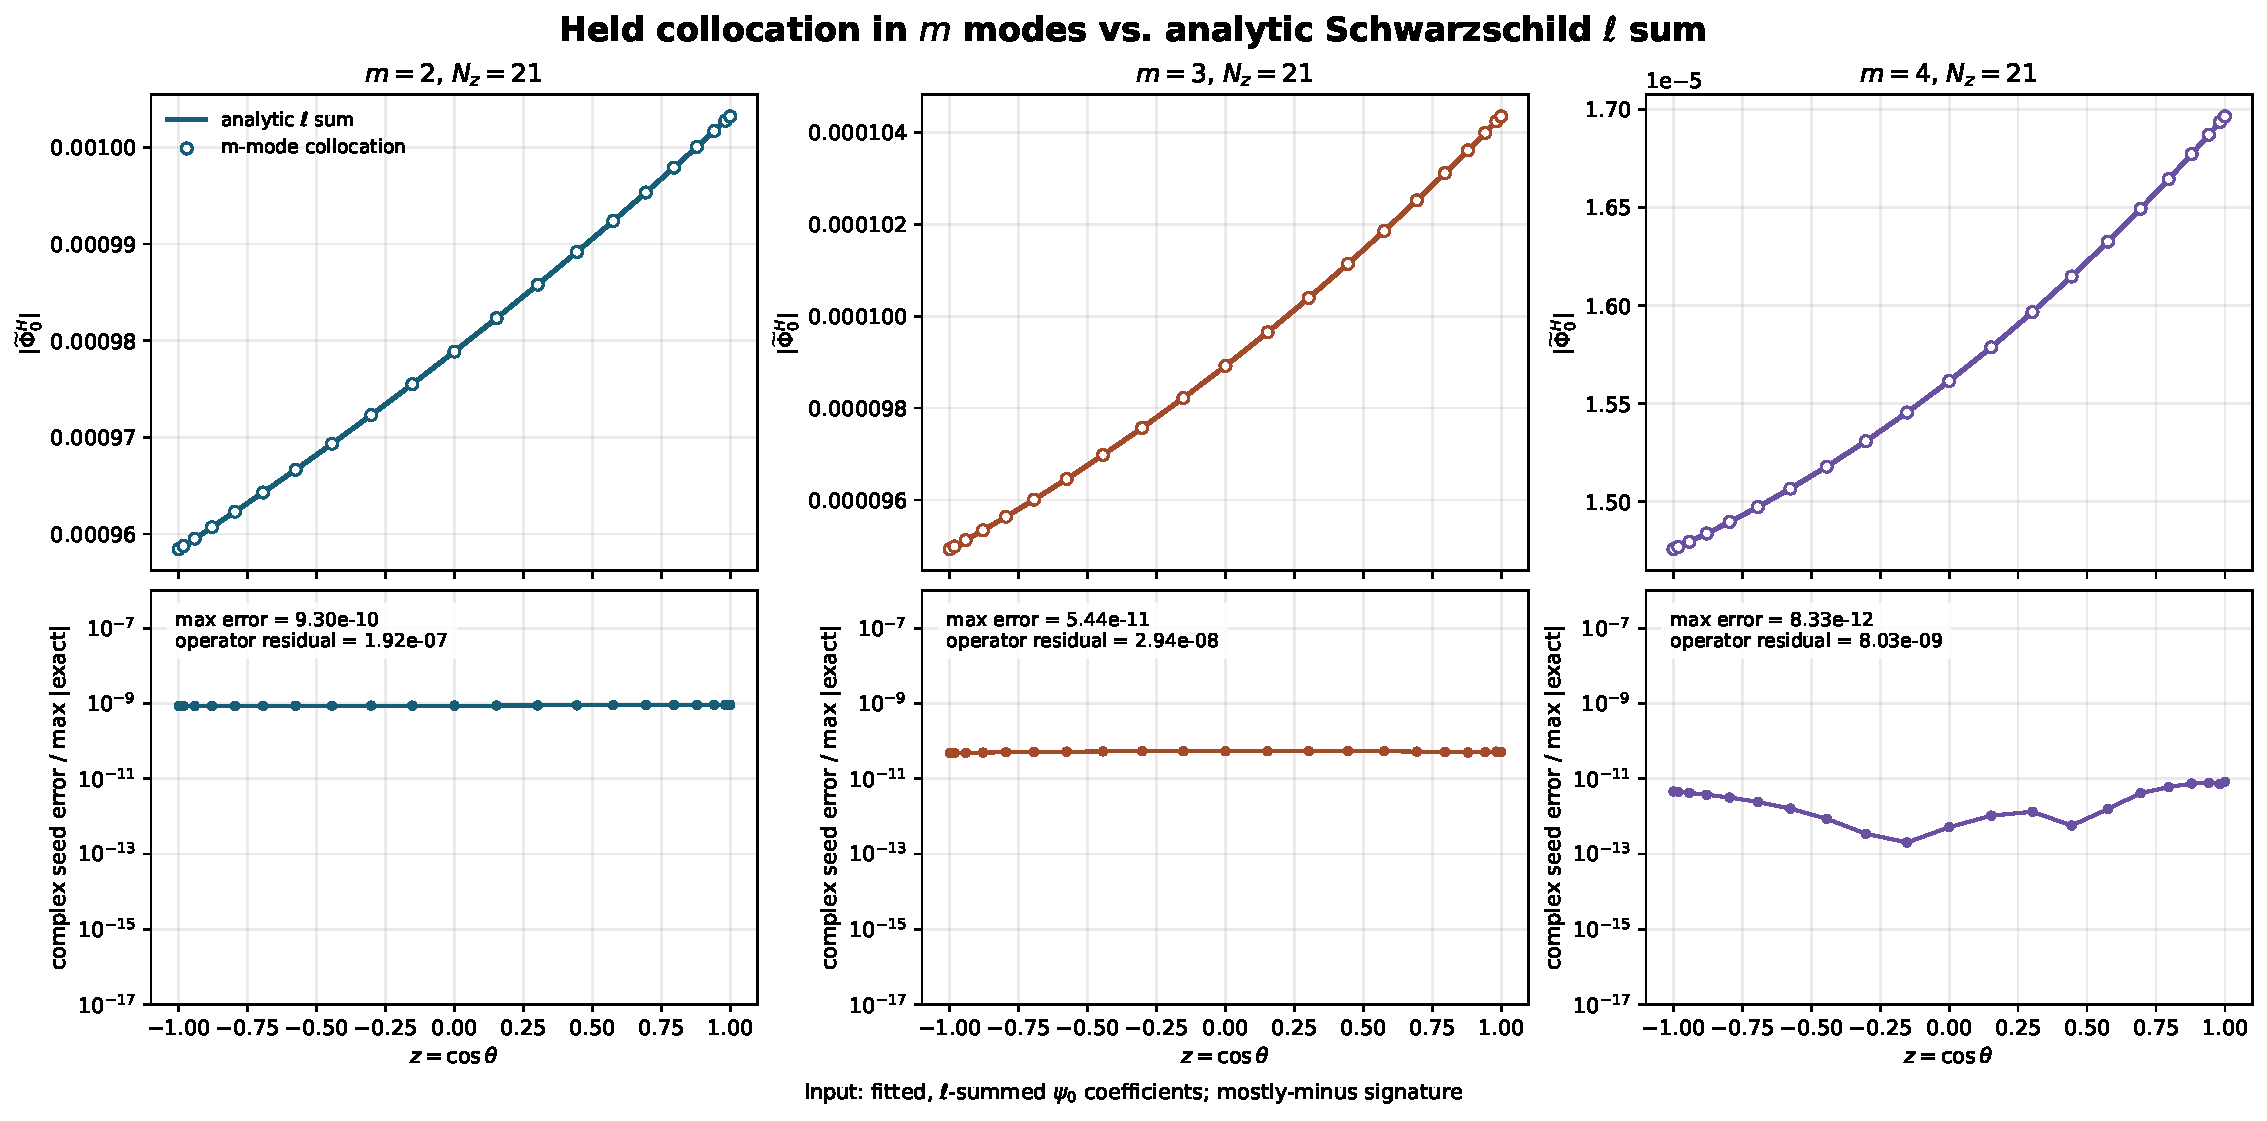
\includegraphics[width=\textwidth]{figures/m_mode_held_collocation.pdf}
  \caption{Validation of the $m$-mode Held seed. Top row: the modulus of the
  reduced seed $\widetilde{\Phi}^{0\circ}$ on the $N_{z}=21$ LGL grid
  (circles), obtained by solving \eqref{eq:reduced eth} in $z$, against the
  analytic Schwarzschild $\ell$ sum (solid). Bottom row: the pointwise complex
  error relative to $\max|\text{exact}|$. The quoted operator residual is the
  relative residual of the reduced angular equation when the analytic seed is
  substituted, and measures the discretization rather than the solve.}
  \label{fig:mmode seed}
\end{figure*}

\emph{Seed inversion.} Figure~\ref{fig:mmode seed} compares the collocation
solution of the reduced angular equation \eqref{eq:reduced eth} with the
analytic $\ell$-summed seed for $m=2,3,4$. The maximum relative complex seed
errors are $9.30\times10^{-10}$, $5.44\times10^{-11}$ and
$8.33\times10^{-12}$, with relative operator-equation residuals for the
analytic seed of $1.92\times10^{-7}$, $2.94\times10^{-8}$ and
$8.03\times10^{-9}$. The errors fall steeply with $m$, as expected from the
pole factorization \eqref{eq:pole factor}: the residual function $\hat X$
becomes smoother as $|m|$ grows, so the spectral representation converges
faster. The equilibrated condition number of the discrete operator falls
correspondingly, from $8.6\times10^{7}$ at $m=2$ to $4.9\times10^{5}$ at
$m=4$, which is why the equilibrated full-pivot solve with iterative
refinement is used rather than a plain factorization. This validates both the
$\ell$-summed input and the $m$-mode seed inversion.

\begin{figure*}
  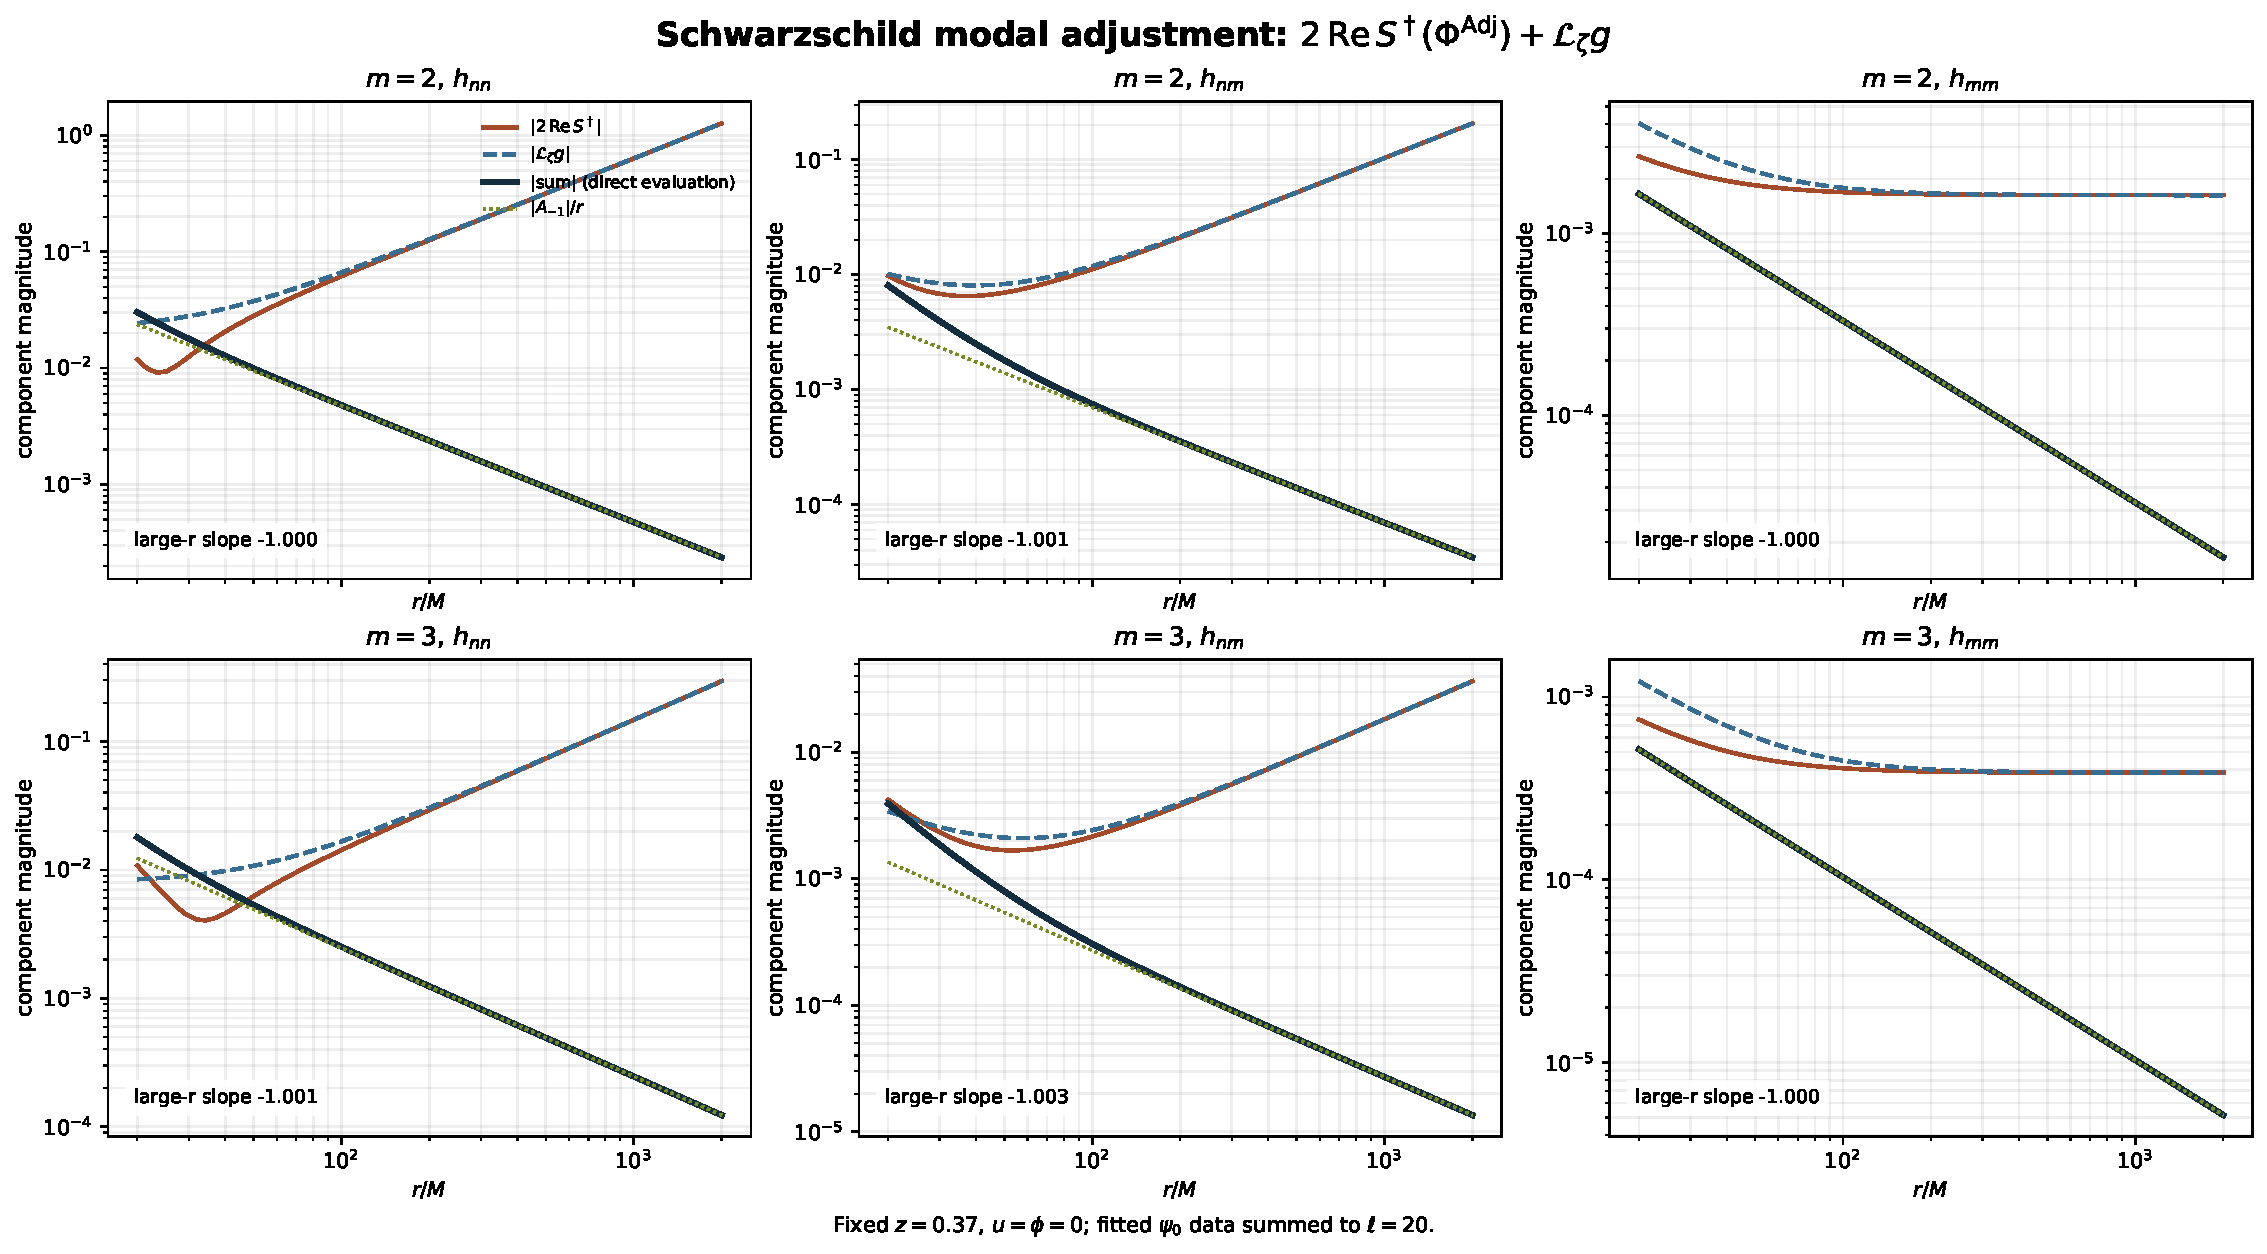
\includegraphics[width=\textwidth]{figures/adjusted_metric_radial_falloff.pdf}
  \caption{Independent modal reference for the adjustment
  \eqref{eq:habadjusted}, built from the closed-form Schwarzschild $(\ell,m)$
  components summed at fixed $m$ through $\ell=20$, evaluated at
  $z=0.37$, $u=\varphi=0$. Each panel shows the reconstructed piece
  $|2\Re\S^{\dagger}\Phi^{\rm Adj}|$, the gauge piece $|\Lie_{\zeta}g|$, their
  sum, and the fitted $|A_{-1}|/r$ Laurent coefficient. The individually
  growing pieces cancel to leave a $1/r$ tail.}
  \label{fig:modal falloff}
\end{figure*}

\emph{Cancellation and Bondi falloff.} The central claim of
Sec.~\ref{sec:scheme} is that the $r^{3}$ and $r^{2}$ terms carried separately
by $2\Re\S^{\dagger}\Phi^{\rm Adj}$ and by $\Lie_{\zeta}g_{ab}$ cancel in the
sum \eqref{eq:habadjusted}, leaving a perturbation with Bondi-like falloff.
Figure~\ref{fig:modal falloff} exhibits this cancellation in the modal
reference. Across $1254$ nonstationary radiative mode components through
$\ell=20$, the largest relative cancellation error in the growing and constant
Laurent coefficients is $4.90\times10^{-16}$, i.e.\ at the level of double
precision. Direct finite-radius sums at $z=0.37$ for $m=2,3$ show $h_{nn}$,
$h_{nm}$ and $h_{mm}$ approaching $1/r$ between $r=20M$ and $r=2000M$, with
fitted large-radius slopes between $-1.003$ and $-1.000$. The residual drift
from $-1$ is the expected contamination from the subleading $\log r/r^{2}$ and
$1/r^{2}$ terms at finite radius, and shrinks as the fitting window is pushed
outward.

\begin{figure*}
  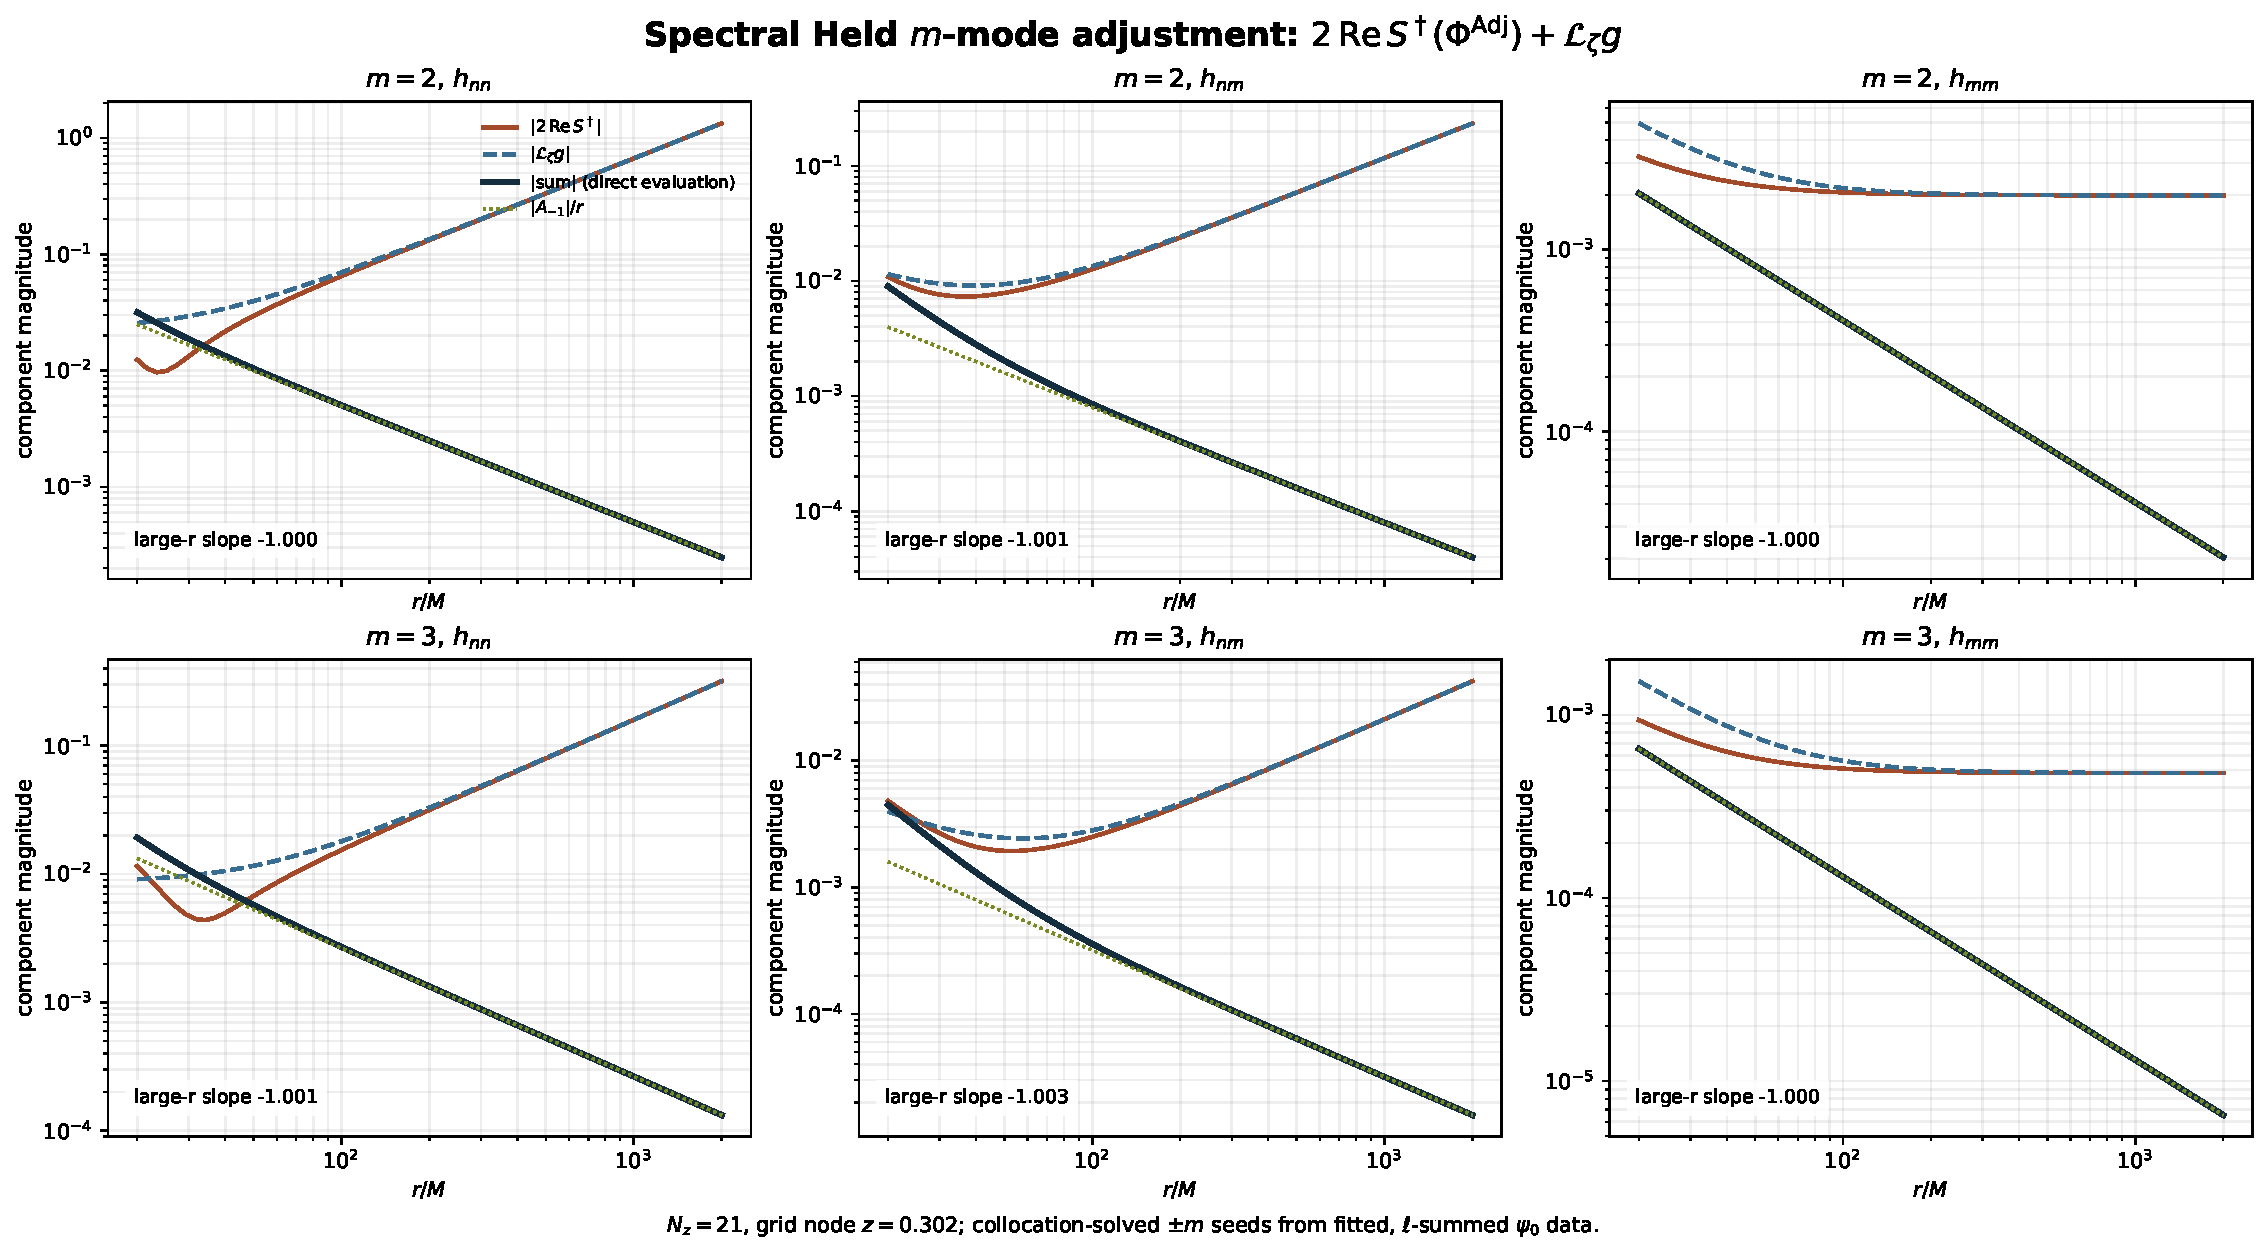
\includegraphics[width=\textwidth]{figures/spectral_m_mode_metric_falloff.pdf}
  \caption{The same six components as Fig.~\ref{fig:modal falloff},
  reconstructed instead from the collocation-solved $\pm m$ Held seeds on the
  $N_{z}=21$ grid and evaluated at the interior node $z=0.3020$. The
  reconstruction forms $\Phi^{0\circ}$ through $\Phi^{3\circ}$, applies the
  spectral Held angular derivatives for $\S^{\dagger}$ and $\Lie_{\zeta}g$,
  and sums the complex Laurent coefficients directly at each radius, without
  ever projecting back onto individual $(\ell,m)$ modes.}
  \label{fig:spectral falloff}
\end{figure*}

\emph{The spectral operator chain.} Figure~\ref{fig:spectral falloff} repeats
the radial test with the full $m$-mode pipeline in place of the modal
reference: the $+m$ and $-m$ seeds are obtained by collocation, the reflected
partner being the conjugate of the reduced $-m$ seed since the angular
harmonics already supply the odd-$m$ reflection phase, and all subsequent
angular derivatives are taken spectrally. At the interior node
$z=0.3020$ the six plotted components again have large-radius slopes between
$-1.003$ and $-1.000$. Across all interior nodes the largest relative
difference from the modal reference of Fig.~\ref{fig:modal falloff} is
$1.04\times10^{-6}$ for $m=2$ and $1.54\times10^{-7}$ for $m=3$, while the
largest relative residual in the growing and constant Laurent coefficients is
$2.24\times10^{-12}$. The cancellation is therefore not an artifact of the
mode sum: it survives the spectral realization of the Held operators, which is
the only form available in Kerr.

\begin{figure*}
  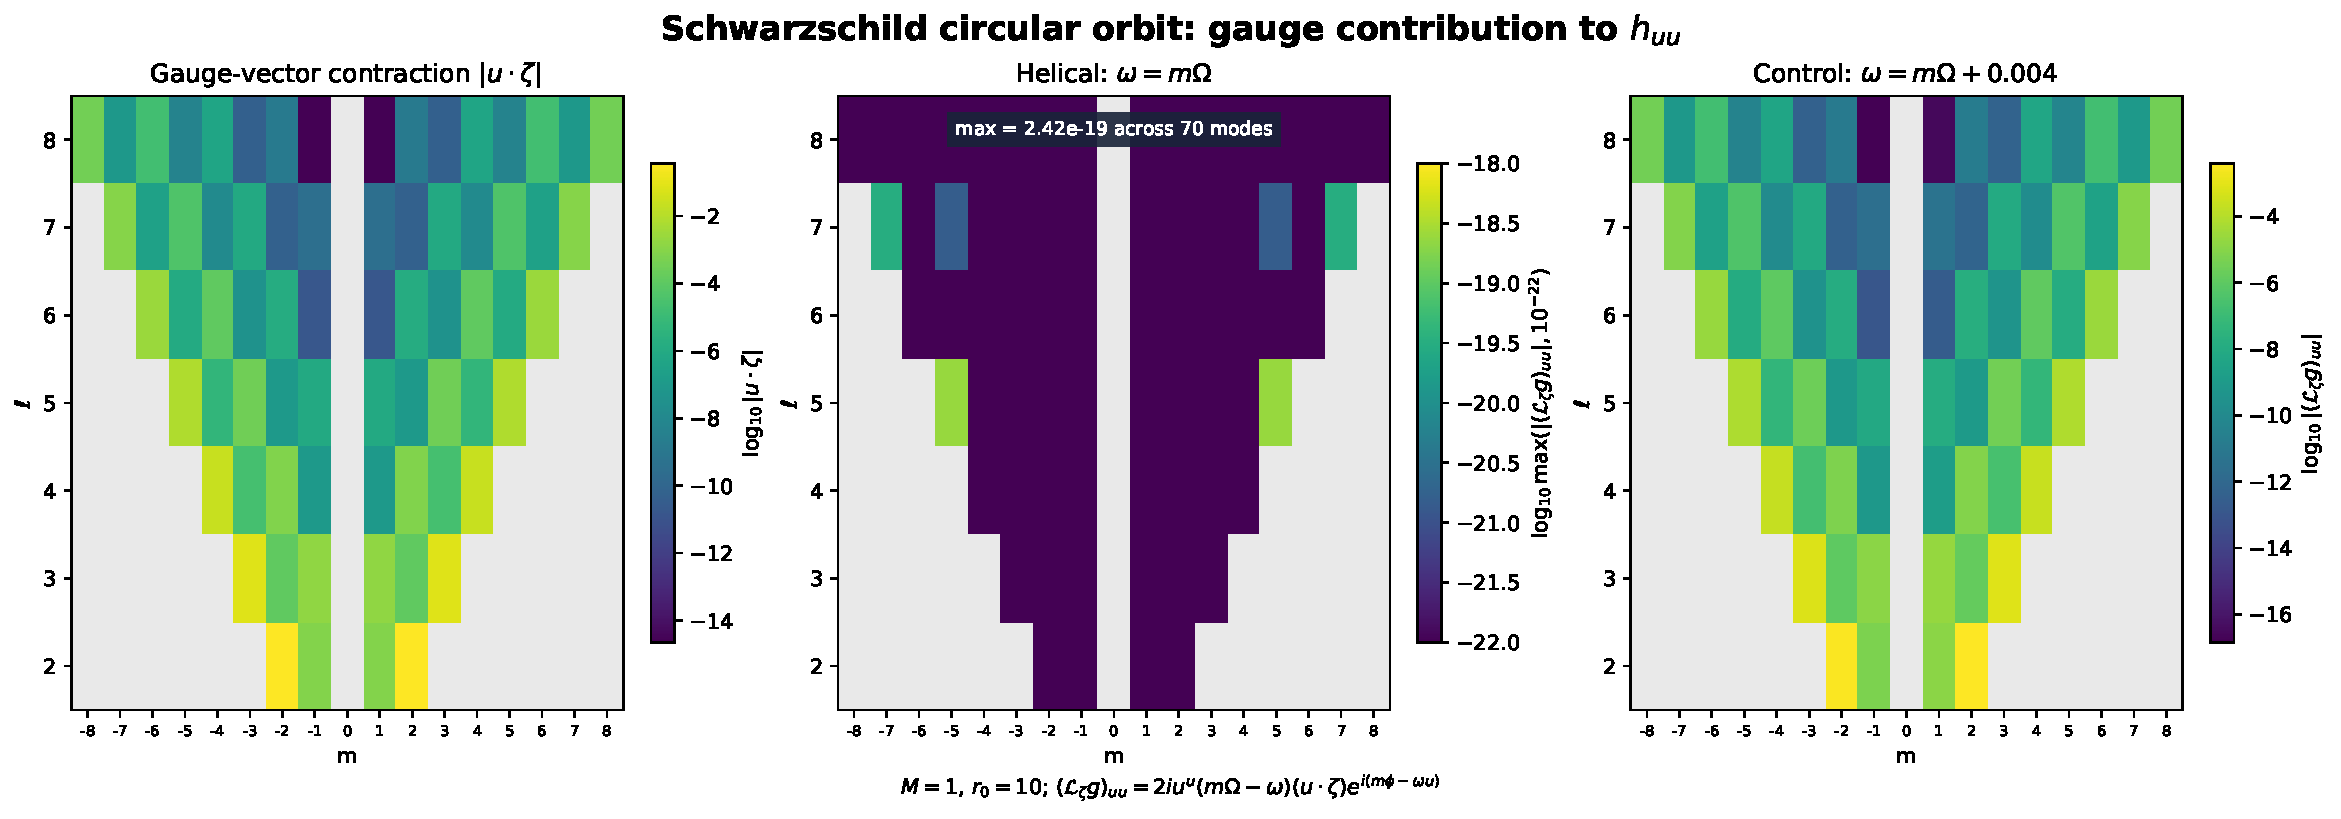
\includegraphics[width=\textwidth]{figures/lie_zeta_redshift_modes.pdf}
  \caption{Gauge contribution to $h_{uu}$ for the Schwarzschild circular
  orbit, over $70$ modes with $2\le\ell\le8$ and $m\neq0$. Left: the worldline
  contraction $|u\cdot\zeta|$, which is generically nonzero. Center: the
  helical pullback $|u^{a}u^{b}(\Lie_{\zeta}g)_{ab}|$ evaluated on shell at
  $\omega=m\Omega_{\varphi}$. Right: the same quantity detuned to
  $\omega=m\Omega_{\varphi}+0.004$. Color scales are $\log_{10}$ and differ
  between panels.}
  \label{fig:lie zeta}
\end{figure*}

\emph{Gauge contribution at the particle.} The quantity of physical interest
at the worldline is $h_{uu}$, to which the residual gauge vector contributes
through $u^{a}u^{b}(\Lie_{\zeta}g)_{ab}$. For a circular geodesic the modal
formula carries an explicit factor of $(m\Omega_{\varphi}-\omega)$, so this
contraction must vanish identically on shell even though $u\cdot\zeta$ itself
does not. Figure~\ref{fig:lie zeta} confirms this: over $70$ modes the maximum
helical value is $2.42\times10^{-19}$, at roundoff, while $|u\cdot\zeta|$
ranges over some twelve decades in the same modes. Detuning the frequency by
$\delta\omega=0.004$ raises the maximum to $3.93\times10^{-3}$, confirming
that the null result is the $(m\Omega_{\varphi}-\omega)$ identity and not an
accidental cancellation or a quantity that was never computed. This checks the
gauge-vector contraction only, and is not by itself a validation of the full
$h_{uu}$, which also requires the corrector $x_{uu}$ of
Sec.~\ref{sec:corrector}.

\PZ{Three things on this subsection. (i) the numbers quoted above are read off the
plotting \texttt{README} and \texttt{m\_mode\_summary.csv}. The condition
numbers and the $m$-scaling remark may be deleted. (ii) The original \emph{retarded} Hertz
metric is not shown in any of these figures, only the adjusted one. (iii) As flagged above, everything here is $a=0$. }

\subsection{Remarks on $(\ell,m)$-mode scheme in Kerr}
\label{sec:lm kerr}

For moderately inclined and eccentric orbits an $(\ell,m)$-mode treatment
remains attractive, since every step of our scheme other than the Teukolsky
solve itself stays algebraic. We summarize here what changes relative to the
Schwarzschild case of Sec.~\ref{sec:schw}.

A generic bound geodesic has three fundamental frequencies, and any
spin-$s$ quantity is expanded as
\begin{equation}\label{eq:modeexp generic}
  {}_s X = \sum_{\ell \emm n k} {}_s X_{\lmnk}(r)\,
  \sSS{s}{\ell}{\emm}(\theta;a\wmnk)\,
  e^{-i\wmnk u + i\emm\varphi_*},
\end{equation}
in place of \eqref{eq:modeexp}, where
$\wmnk = \emm\Omega_{\varphi} + n\Omega_{r} + k\Omega_{\theta}$. The asymptotic amplitudes
$\psifiveM{\lmnk}$ are the $\scri$ amplitudes of the $s=+2$ point-particle
Teukolsky solution and require no new radial integrations beyond those
already performed. Only the canonical half of the $(\emm,n,k)$ lattice need
be computed, the remainder following from the polar reflection symmetry of
the spheroidal functions,
\begin{equation}\label{eq:Z symmetry generic}
  \Zinf{s}{\ell,-\emm,-n,-k} = (-1)^{\ell+k}\,\big(\Zinf{s}{\lmnk}\big)^{*} .
\end{equation}

In practice we do not solve the radial Teukolsky equation ourselves in this
scheme. The seed data are obtained from the publicly available Julia package
\textsc{GeneralizedSasakiNakamura.jl}~\cite{Lo:2023fvv,GSNjl}, which integrates
the frequency-domain radial Teukolsky equation for Kerr in its generalized
Sasaki--Nakamura form. Transforming to the GSN variable removes the long-range
part of the Teukolsky potential, so that the asymptotic behaviour is reached at
moderate radii and the $\scri$ and horizon amplitudes are extracted from
short-range solutions rather than from slowly convergent series; this is
precisely the quantity our scheme consumes, and it is the numerically delicate
one at small $\wmnk$ and large $\ell$. The package covers $s=0,\pm1,\pm2$ and
arbitrary $a$, uses \textsc{SpinWeightedSpheroidalHarmonics.jl} for the angular
problem, and supplies point-particle amplitudes for generic bound orbits
parametrized by $(p,e,x)$, from which the lattice of frequencies $\wmnk$ and the
corresponding $\Zinf{+2}{\lmnk}$ follow directly. For each mode of the canonical
half-lattice we take the $\scri$ amplitude returned by the package, convert it
to our conventions, and identify it with $\psifiveM{\lmnk}$; the $(\ell,\emm)$
data are then piped into the pipeline of Sec.~\ref{sec:schw}, entering as the
seed \eqref{eq:f mode kerr} of the Held hierarchy. Nothing else in the scheme is
sensitive to how the radial problem was solved, so the package may be replaced
by any code returning amplitudes in the same normalization.
\PZ{Two things to check: (i) the overall convention/normalization map between
the package's \texttt{Amplitudes["I"]} and our $\psifiveM{\lmnk}$ --- signature
and the $\rho^{-4}$ scaling both enter; (ii) the package documentation lists an
additional citation for the point-particle/inhomogeneous solutions on top of
\cite{Lo:2023fvv}.}

The HMS is unchanged in form. On a mode $\thpH\to-i\wmnk$, and the eighth-order
angular operator in \eqref{eq:f seed} is precisely the combination appearing in
the Teukolsky--Starobinsky identities, so it is diagonalized by the spheroidal
harmonics and \eqref{eq:f mode kerr} continues to hold with $\Dlw$ the Kerr
Teukolsky--Starobinsky constant. Everything downstream of the seed is likewise
unchanged as a set of Held equations. What changes is that these equations are
no longer diagonal in $\ell$, and there are exactly three sources of mixing.

First, the seed is produced in the spheroidal basis, whereas Held's angular
derivatives act simply on spin-weighted \emph{spherical} harmonics. We
therefore expand
\begin{subequations}\label{eq:spheroidal to spherical}
\begin{align}
  \sSS{s}{\ell}{\emm}(\theta;a\omega)
  &= \sum_{L} b^{(s,\ell,\emm)}_{L}(a\omega)\,\sYY{s}{L}{\emm}(\theta),
  \label{eq:b coeffs}\\
  \fHo_{L\emm n k}
  &= \sum_{\ell} \fHo_{\lmnk}\,b^{(+2,\ell,\emm)}_{L}(a\wmnk),
  \label{eq:f Y basis}
\end{align}
\end{subequations}
and work in the spherical basis thereafter. The mixing coefficients depend
only on $(s,\ell,\emm,a\omega)$ and are computed once per mode and cached,
since every Held chain downstream reuses them.

Second, $\edthH$ and $\edthpH$ acquire off-diagonal pieces proportional to
$a\omega$, and the multiplication operators $\tah$, $\tabh$ and $\Oh$ ---
which vanish identically when $a=0$ --- are themselves off-diagonal. All five
are tridiagonal in $\ell$ at fixed $\emm$.

Third, $\rho^{-1} = -(r - ia\cos\theta)$ is no longer a multiple of the
identity. Using
\begin{equation}\label{eq:cos theta rec}
  \cos\theta\;\sYY{s}{\ell}{\emm}
  = c_{\ell+1}\,\sYY{s}{\ell+1}{\emm} + b_{\ell}\,\sYY{s}{\ell}{\emm}
  + c_{\ell}\,\sYY{s}{\ell-1}{\emm},
\end{equation}
with
\begin{equation}\label{eq:cos theta coeffs}
  c_{\ell}(s,\emm)=\sqrt{\frac{(\ell^{2}-\emm^{2})(\ell^{2}-s^{2})}
  {\ell^{2}(4\ell^{2}-1)}},
  \qquad
  b_{\ell}(s,\emm)=-\frac{s\,\emm}{\ell(\ell+1)},
\end{equation}
the operator $\rho^{-1}$ is the tridiagonal matrix
$\mathsf R = -r\,\mathbb{1} + ia\,\mathsf C$, where $\mathsf C$ is the matrix
of \eqref{eq:cos theta rec}, and the adjusted Hertz potential
\eqref{eq:Phi completion intro} is evaluated in Horner form,
\begin{equation}\label{eq:Phi adj horner}
  \boldsymbol{\Phi}^{\rm adj}
  = \boldsymbol{\Phi}^{0\circ}
  + \mathsf R\Big(\boldsymbol{\Phi}^{1\circ}
  + \mathsf R\big(\boldsymbol{\Phi}^{2\circ}
  + \mathsf R\,\boldsymbol{\Phi}^{3\circ}\big)\Big),
\end{equation}
as a vector over $\ell$ at fixed $(\emm,n,k)$. It is worth noting that the
same matrix $\mathsf C$ also represents $\Oh = -2ia\cos\theta$, so the second
and third sources of mixing share their only nontrivial ingredient.

Since each of the five angular operators is tridiagonal, a chain of $p$ of
them is banded with half-bandwidth $p$. The longest chain is the
$\edthpH^{\,3}\edthH^{\,3}$ appearing in $\PhiN{0}$, and
\eqref{eq:Phi adj horner} adds at most three further neighbours, so
$\Phiadj$ at output multipole $L$ requires the seed out to $\ell \le L+6$,
and the seed in turn requires spheroidal amplitudes out to
$\ell\le L+6+N_{\rm mix}$, where $N_{\rm mix}$ is the half-width at which
\eqref{eq:b coeffs} is truncated. The cost of the completion
is then $O(L_{\max})$ per $(\emm,n,k)$, which is negligible beside the
radial Teukolsky solves that produce its input.

Finally, the two schemes can be compared directly: the $(\ell,m)$-mode
amplitudes may be resummed onto the same $(r,z)$ grid used in
Sec.~\ref{sec:mmode HMS} through
\begin{equation}\label{eq:ell resum}
  {}_sX_{\omega\emm}(r,z)
  = \sum_{\ell} {}_sX_{\lmnk}(r)\,
    \sSS{s}{\ell}{\emm}(\arccos z;a\wmnk),
\end{equation}
which provides a mode-by-mode check of the collocation solve against a
calculation that shares none of its angular machinery.

\PZ{This subsection is drafted from
\texttt{BondiGauge\_Adjusted\_Generic.nb} in
\texttt{MathematicaNotebooks/EffectiveSource/lm\_mode}; \eqref{eq:ell resum}
is its \texttt{ellSummedMode}/\texttt{ellSummedModeRZ}.  Open items:
(i) quote the production $(\ell_{\max},n_{\max},k_{\max})$ and the orbit
--- the notebook is currently exploratory at $a=0.667M$, $p=10M$, $e=0.1$,
$\cos\chi=\cos(\pi/4)$, $\ell_{\max}=3$, $n_{\max}=3$, $k_{\max}=4$;
(ii) quote $N_{\rm mix}$ and justify it (the notebook keeps 30 terms with a
$10^{-25}$ chop, which is far more than needed for $a\omega\lesssim1$ --- a
plot of $|b_L|$ against $|L-\ell|$ at the largest $a\wmnk$ in the run would
let you state a much smaller effective value);
(iii) say whether \eqref{eq:Z symmetry generic} is meant for general $s$ or
only $s=+2$, which is all the notebook uses.}

\subsection{Computational cost}

% PZ: this is referred to as "App." in the text and carries the label
% app:Lie, but was being numbered as an ordinary section.
\appendix
\section{Lie derivative of $g_{ab}$ along $\zeta^{a}$}
\label{app:Lie}
% ROADMAP: the long Held expressions.  These are transcribed from Vahid's
% notes eqs (18)-(20).  They are long enough that a transcription error is
% likely -- flag them and check against the notebook's LieZetagComps, which
% is the a = 0 specialisation.
Since $\zeta^a$ is by construction compatible with the traceless IRG, we have $\Lie_{\zeta}g_{ab}l^{a}=0$ and $\Lie_{\zeta}g_{ab}m^{a}\bar m^{b}=0$. 
The remaining, non-zero, NP components are
\begin{widetext}
\begin{align}
\left(\Lie_{\zeta}g \right)_{mm} 
&=
-2\bar\rho\,\edthH\edthH\zetal
+2\edthpH\edthH\fHo
+2\Oh\thpH\fHo
+4\bar\rho\,\tah\,\edthpH\fHo
+8\rhopH\fHo ,
\label{eq:Lie mm}
\end{align}
\begin{align}
\left(\Lie_{\zeta}g\right)_{nm}
&=
\bar\rho\,\edthpH\edthH\edthH\zetal
-2\rho\bar\rho\,\tabh\,\edthH\edthH\zetal
+\rho(\rho+\bar\rho)\Psih\,\edthH\zetal
-\bar\rho\,\Oh\,\edthpH\edthpH\edthH\fHo
+2\rho\,\tabh\,\edthpH\edthH\fHo
\non\\
&\quad
+\frac{1}{\bar\rho}\Big(
-2\bar\rho\,\Oh{}^{2}\,\edthpH\thpH\fHo
+2(\rho+\bar\rho)\Oh\tabh\,\thpH\fHo
-2\bar\rho\,\tah\,\edthpH\edthpH\fHo
-(\rho^{2}\Oh+\rho)\Psih\,\edthpH\fHo
\Big)
\non\\
&\quad
+\bar\rho\,\Psibh\,\edthpH\fHo
-6\bar\rho\,\Oh\rhopH\,\edthpH\fHo
+4\rho\bar\rho\,\tah\tabh\,\edthpH\fHo
+8\rho\rhopH\tabh\,\fHo ,
\label{eq:Lie nm}
\end{align}
and
\begin{align}
\left(\Lie_{\zeta}g \right)_{nn}
&=
\Re\Bigg[
4\rho\bar\rho\,\tabh\,\edthpH\edthH\edthH\zetal
-4\rho^{2}\bar\rho\,\tabh{}^{2}\,\edthH\edthH\zetal
+2\rho^{2}\Psih\,\edthpH\edthH\zetal
+4\rho^{2}\bar\rho\,\Psih\tabh\,\edthH\zetal
\non\\
&\qquad
-2\edthpH\edthpH\edthpH\edthH\fHo
-\frac{2}{\rho}\Big(
4\Oh\,\edthpH\edthpH\thpH\fHo
-4\rho\bar\rho\,\Oh\tabh\,\edthpH\edthpH\edthH\fHo
+4\big(4+\bar\rho\,\Oh-\rho\bar\rho\,\Oh{}^{2}\big)\tabh\,\edthpH\thpH\fHo
\Big)
\non\\
&\qquad
-\big(8\rhopH+3\rho\Psih+3\bar\rho\Psibh+2\rho^{2}\Oh{}^{2}\Psih
+8\rho\bar\rho\,\tah\tabh\big)\edthpH\edthpH\fHo
+4\rho^{2}\tabh{}^{2}\,\edthpH\edthH\fHo
+4\rho(\rho+2\bar\rho)\Oh\tabh{}^{2}\,\thpH\fHo
\non\\
&\qquad
+8\rho^{2}\bar\rho\,\tah\tabh{}^{2}\,\edthpH\fHo
+4\rho\bar\rho\,\Psibh\tabh{}^{2}\,\edthpH\fHo
-24\rho\bar\rho\,\Oh\rhopH\tabh\,\edthpH\fHo
+16\rho^{2}\rhopH\tabh{}^{2}\,\fHo
\Bigg].
\label{eq:Lie nn}
\end{align}
The remaining components follow by conjugation,
$\Lie_{\zeta}g_{ab}n^{a}\bar m^{b}=\overline{\Lie_{\zeta}g_{ab}n^{a}m^{b}}$
and
$\Lie_{\zeta}g_{ab}\bar m^{a}\bar m^{b}=\overline{\Lie_{\zeta}g_{ab}m^{a}m^{b}}$,
which in mode space are 
\begin{equation}\label{eq:Lie conj modes}
\big(\Lie_{\zeta}g\big)_{n\bar m, \omega \ell m}
= -(-1)^{\emm}\,\overline{
\big(\Lie_{\zeta}g\big)_{nm, -\omega \ell -m}
},
\qquad
\big(\Lie_{\zeta}g\big)_{\bar m\bar m,\l\emm}
= (-1)^{\emm}\,\overline{\big(\Lie_{\zeta}g\big)_{mm,-\omega \ell -m}} .
\end{equation}
\end{widetext}
The relative minus sign between the two is the $(-1)^{s}$ arising when conjugating a spin-weighted harmonic.


\clearpage
	\bibliographystyle{apsrev4-2}
\bibliography{MyReferences,bghz_extra}


\section{Teukolsky operators in Held form}
\label{app:Teuk}

For $\psi_{0}$ the Teukolsky wave operator in \eqref{eq:Teuksource} reads, in
Held form,
\begin{widetext}
\begin{align}\label{eq:TeukO Held}
\half \mathcal O \psi_{0}
&= \half\,\rho\bar\rho\,(3\PsiH\rho + 8\rhopH)\,\psi_{0}
 - \half\Big(\PsiH\rho\,(3\rho+\bar\rho) + 2\bar\rho\,\rhopH
   + \rho\bar\rho\big(-\PsibH + 6\rho\,\tauH\taubH
   + (\rhopH+\rhopbh)\,\Oh\big)\Big)\,(\th\psi_{0})
\non
&\quad
+ \th\thpH\psi_{0}
+ \rho\bar\rho\,\taubH\,(\th\Dbar\,\psi_{0})
+ \rho\bar\rho\,\tauH\,(\th\Dbar'\psi_{0})
- (4\rho+\bar\rho)\,(\thpH\psi_{0})
- \rho\bar\rho\,(\Dbar\Dbar'\psi_{0}),
\end{align}
and the source is
\begin{align}\label{eq:Teuk T0 Held}
T_{0} &= 2\bar\rho\,(-2\rho+\bar\rho)\,\tauH\,(\th T_{lm})
 - 4\rho\,(\th T_{mm}) - \th\th T_{mm}
\non
&\quad + \bar\rho\Big(
 2T_{mm}(2\rho+\bar\rho)
 + 4\bar\rho^{2}\,\tauH\big(T_{lm} + T_{ll}(\rho-\bar\rho)\,\tauH\big)
 + \th\Dbar T_{lm}
 + 4\bar\rho\,(-\rho+\bar\rho)\,\tauH\,(\Dbar T_{ll})
\non
&\qquad\quad
 - 2(2\rho+\bar\rho)\,(\Dbar T_{lm})
 + \Dbar\th T_{lm}
 - \bar\rho\,(\Dbar\Dbar T_{ll})
\Big).
\end{align}
\end{widetext}
Both are written with the barred and unbarred Held scalars kept distinct, and
we have used $[\th,\Dbar]=0$ in \eqref{eq:Teuk T0 Held}.

In the retarded outgoing chart the coefficients of \eqref{eq:Teuk ABC} are
\begin{widetext}
\begin{subequations}\label{eq:Teuk ABC coeffs}
\begin{align}
 \hat A &= -\Delta \rho\bar\rho, \\
     \hat B &= -\left(\PsiH\rho(3\rho+\bar\rho)+2\bar\rho\rhopH+\rho\bar\rho(-\PsibH+6\rho\tauH\taubH+\Held\Omega(\rhopH+\bar\rhopH))\right)\non
     &\quad +2\rho\bar\rho( \taubH \Dbar + \tauH \Dbar'), \\
     \hat C &=  \pd_r(\Delta \rho\bar\rho) -(4\rho+\bar\rho)\pd_u +\frac12 \rho\bar\rho \left(3\PsiH \rho + 8 \rhopH\right)  -\rho\bar\rho\Dbar\Dbar'.
\end{align}
\end{subequations}
\end{widetext}
The terms containing $\Delta$ are the price of the retarded chart: they arise
because $n^{\mu}$ has a component along $r$,
$n^{\mu}\pd_{\mu}r = -\Delta/(2\Sigma)$, and they are the only
non-Held-covariant pieces.

\end{document}
